%! Mode:: "TeX:UTF-8"
%! TEX program = xelatex
% A题 LaTeX 论文 —— 锂电池剩余寿命预测与梯次利用筛选优化
% 编译方式: xelatex 编译两遍 (配合 bibtex)
\PassOptionsToPackage{quiet}{xeCJK}
\documentclass[withoutpreface]{cumcmthesis}
\usepackage{etoolbox}
\usepackage{ctex}
\BeforeBeginEnvironment{tabular}{\zihao{-5}}
\usepackage[numbers,sort&compress]{natbib}  % 文献管理宏包
\usepackage{url}
\usepackage{subcaption}
\usepackage{tikz}
\usetikzlibrary{shapes.geometric, arrows.meta, positioning}
\newcolumntype{C}{>{\centering\arraybackslash}X}
\newcolumntype{R}{>{\raggedleft\arraybackslash}X}
\newcolumntype{L}{>{\raggedright\arraybackslash}X}

\title{基于多因子退化机理与数据驱动的锂电池剩余寿命预测及梯次利用优化}

% 封面信息(以无承诺书模式输出, 正式提交前填写; @ 命令需 makeatletter)
\makeatletter
\renewcommand{\mcm@tokens@tihao}{A}
\renewcommand{\mcm@tokens@baominghao}{待填}
\renewcommand{\mcm@tokens@schoolname}{待填}
\renewcommand{\mcm@tokens@membera}{成员A}
\renewcommand{\mcm@tokens@memberb}{成员B}
\renewcommand{\mcm@tokens@memberc}{成员C}
\renewcommand{\mcm@tokens@supervisor}{待填}
\renewcommand{\mcm@tokens@yearinput}{2026}
\renewcommand{\mcm@tokens@monthinput}{8}
\renewcommand{\mcm@tokens@dayinput}{11}
\makeatother

\begin{document}
\pagenumbering{gobble}
\maketitle

\begin{abstract}

\textbf{针对问题一（退化特征分析与影响因子辨识）：}建立了"多维特征体系 + 三阶段划分 + 因子量化"的综合分析框架。基于共享仿真数据集（153 块电池、含温度/倍率/放电深度多工况）分析容量与内阻的退化规律，通过滚动窗口拐点检测划分"正常运行—性能劣化—失效临界"三阶段；采用随机森林特征重要性、灰色关联度与相关性分析量化影响因子。结果表明：温度是首要核心因子（RF 重要性 0.56，平均寿命随温度由 1218 循环（10°C）降至 206 循环（45°C）），倍率次之（0.33），放电深度在老化后期作用上升，各因子经机理链（SEI 生长、析锂、LAM）与宏观退化现象耦合。

\textbf{针对问题二（SOH 评估与 RUL 预测建模）：}构建"多特征融合 SOH 辨识 + 剩余寿命外推"的组合模型。以容量保持率定义 $SOH(t)=Q(t)/Q_{rated}$，对容量序列做滑动平均并给出 95\% 置信带；以退役判定点（SOH=0.80）为起点，对比线性外推、二阶多项式、指数拟合与随机森林四种模型外推至 EOL（70\%）。结果显示二阶多项式拟合 RMSE 最优（0.037），全批退役电池剩余寿命均值约 149 循环、标准差 117 循环。

\textbf{针对问题三（梯次筛选与储能编组优化）：}建立"规则分级 + K-means 聚类 + 多目标编组优化"流程。按统一分级标准（SOH 单指标）对退役电池分级，因退役点 SOH 高度同质（0.82~0.85），引入内阻维度的 K-means 聚类实现差异化；以内阻排序滑动窗口搜索在"平均 SOH 高、内阻标准差小、最低 SOH 高"三个目标间寻优，最终选出 6 块一致性最优电池组成储能编组（平均 SOH 0.8467，内阻标准差 0.0005），并输出 \texttt{selected\_batteries.csv} 供工程配置。

\textbf{针对问题四（多工况仿真与鲁棒性）：}对长期高温（SOH×0.94）、大倍率充放电（内阻×1.2）两类恶劣工况进行仿真，考察编组方案鲁棒性；对筛选阈值、目标权重做单参数灵敏度分析。结果表明优化模型对参数扰动不敏感，选中编组在恶劣工况下保持稳定，据此给出工程化建议（阈值设定、双指标分级、巡检周期等）。

最后，我们对模型进行误差分析与适用性评价，给出改进与推广方向。全文所有数据字段、命名与接口严格符合《数据格式规范 v1.1》，代码与数据已在仓库中随论文发布。

\keywords{锂电池退化；健康状态评估；剩余寿命预测；梯次利用；多目标优化；随机森林}

\end{abstract}

\pagenumbering{arabic}

\section{问题重述}

\subsection{问题背景}
动力锂电池经长期循环后出现容量衰减、内阻升高、性能退化等老化现象，这一过程并非线性可控，而是受多种因素耦合影响。随着我国新能源汽车保有量持续攀升，动力电池报废量逐年增加，退役电池的规模化处置已成为行业亟需解决的问题。退役电池虽仍具备储能潜力，可梯次应用于电网储能、低速交通工具、基站备电等场景，但由于充放电倍率、环境温度、循环次数、放电深度、充电策略等多因素耦合作用，其老化过程具有非线性、随机性与时变性，难以直接沿用新电池的检测与评估体系。据此我们认识到：科学识别老化特征、量化影响因子、评估剩余寿命并合理筛选编组，是保障梯次利用安全性、经济性与一致性的关键前提。由于本题不提供原始实测数据，我们需自主构建合理的仿真时序数据与参数体系，并说明取值依据。

\subsection{问题梳理}
本题由四个层层递进的问题构成，我们将其梳理为一条完整的分析链：问题1 摸清退化规律与关键成因，回答"电池如何老化、什么因素主导老化"，是全题的机理基础；问题2 在此基础上建立健康状态（SOH）评估与剩余寿命（RUL）预测模型，回答"电池还能用多久"，为筛选提供定量指标；问题3 将预测结果用于退役电池的分级筛选与储能编组，回答"如何选、如何配"，实现梯次利用的应用落地；问题4 检验编组方案在恶劣工况下的鲁棒性并给出工程建议，回答"方案稳不稳、如何落地"，完成从机理到工程的闭环。据此，我们按"数据构建（统一规范）$\to$退化机理分析（问题1）$\to$健康状态与寿命预测（问题2）$\to$筛选与编组优化（问题3）$\to$鲁棒性与建议（问题4）"的主线展开全文，各问题通过统一数据接口表衔接，形成有机整体。

\subsection{问题要求}
\textbf{问题1：}分析锂电池性能退化特征（容量/内阻随循环变化），划分退化阶段，梳理影响因子并定量量化各因子影响权重，甄别核心关键因素。

\textbf{问题2：}构建适配锂电池老化特性的 SOH 评估与剩余寿命（RUL）预测模型，完成模型训练、验证与精度对比，预判不同工况下的衰减趋势，并分析恶劣工况对寿命预测的扰动影响。

\textbf{问题3：}在已知每块退役电池 SOH、内阻与剩余寿命的基础上，建立分级筛选标准，在一致性、安全性与经济性约束下求解最优储能编组方案。

\textbf{问题4：}多工况场景仿真与模型鲁棒性分析，检验编组方案的稳定性，给出可量化的工程优化建议。

\section{问题分析}
本题为"机理分析 + 预测建模 + 多目标优化"的综合题型，四个问题环环相扣、逐层递进。由于每一问的建模目标与数据基础不同，我们对每一问先做思路分析、再建模求解，全文按"数据构建（统一规范）$\to$退化机理分析（问题1）$\to$健康状态与寿命预测（问题2）$\to$筛选与编组优化（问题3）$\to$鲁棒性与建议（问题4）"的主线展开，前后问题通过统一数据接口表（\texttt{battery\_health\_indicators.csv}、\texttt{selected\_batteries.csv}）衔接。技术路线如图 \ref{fig:flow} 所示。

\begin{figure}[H]
\centering
\begin{tikzpicture}[node distance=1.1cm, auto, font=\zihao{-5}]
\tikzstyle{box}=[rectangle, draw=black, thick, fill=blue!8, text width=3.6cm, minimum height=0.9cm, text centered, rounded corners=2pt]
\tikzstyle{arrow}=[->, thick]
\node[box] (d) {仿真数据构建\\（多因子衰减模型）};
\node[box, below=0.55cm of d] (a) {成员A：时序数据\\battery\_timeseries.csv};
\node[box, below=0.55cm of a] (b) {成员B：健康指标表\\battery\_health\_indicators.csv};
\node[box, below=0.55cm of b] (c) {成员C：选中结果表\\selected\_batteries.csv};
\node[box, right=1.6cm of d] (q1) {问题1\\退化特征与因子量化};
\node[box, right=1.6cm of a] (q2) {问题2\\SOH评估与RUL预测};
\node[box, right=1.6cm of b] (q3) {问题3\\梯次筛选与编组优化};
\node[box, right=1.6cm of c] (q4) {问题4\\鲁棒性与工程建议};
\draw[arrow] (d) -- (q1);
\draw[arrow] (d) -- (a);
\draw[arrow] (a) -- (b);
\draw[arrow] (b) -- (c);
\draw[arrow] (q1) -- (q2);
\draw[arrow] (q2) -- (q3);
\draw[arrow] (q3) -- (q4);
\end{tikzpicture}
\caption{全文技术路线与数据流转}\label{fig:flow}
\end{figure}

\subsection{数据预处理的分析}
为得到可信的建模输入，我们首先对仿真数据进行质量检查与规范化处理，并尝试从四个方面入手。首先，核对数据规模、字段完整性与唯一性，确认是否存在缺失值或重复记录；其次，由于容量观测中包含容量再生尖刺与自相关测量噪声，我们需要对其进行识别并在机理建模时予以区分；随后，统一各字段的单位、命名与阶段划分口径，消除跨成员交接时的歧义；最后，基于单调退化趋势派生多维健康特征，为问题1 的退化特征分析提供数据基础。

\subsection{问题一的分析}
问题一要求识别退化特征并甄别核心关键因素，我们将其分解为五步依次推进。首先，构建容量、内阻等多维退化特征体系，通过可视化考察其随循环的变化形态；其次，由于容量衰减存在明显的阶段差异，我们基于拐点理论与滚动斜率检测划分退化三阶段；随后，梳理影响因子清单，并建立"外部因子$\to$内部机理$\to$老化模式$\to$宏观表现"的作用机理链；最后，为定量甄别核心因子，我们采用随机森林特征重要性、相关性分析并辅以灰色关联度与熵权法交叉验证，并结合温度—寿命规律甄别核心关键因素，为问题2/3 提供物理先验。

\subsection{问题二的分析}
问题二要求在问题1 的退化机理之上建立 SOH 评估与 RUL 预测模型。我们考虑从"辨识—外推—量化—扰动"四步展开：首先，以容量保持率定义 SOH，对容量序列做滑动平均平滑并给出 95\% 置信区间；其次，以退役判定点（SOH=0.80）为预测起点，对比线性外推、二阶多项式、指数拟合与随机森林四种外推模型的精度；随后，通过置信带与跨电池统计量化预测不确定性；最后，依据问题1 的机理链对恶劣工况进行参数扰动注入，分析其对寿命预测的扰动影响。

\subsection{问题三的分析}
问题三要求在已知每块退役电池 SOH、内阻与剩余寿命的基础上求解最优储能编组。我们按"提取—分级—优化—输出"四步展开：首先，从健康指标表提取退役电池在退役判定点的状态；其次，由于退役点 SOH 高度同质，我们尝试采用"规则分级 + K-means 聚类"相结合的差异化分级；随后，以平均 SOH 高、内阻离散小、最低 SOH 高为目标构建多目标编组优化模型，采用内阻排序滑动窗口穷举搜索求解；最后，输出满足一致性、安全性与经济性约束的最优编组方案，供工程配置。

\subsection{问题四的分析}
问题四要求检验编组方案在恶劣工况下的鲁棒性并给出工程建议。由于前面得到的编组方案需经受工况变化考验，我们首先构造长期高温与频繁大倍率两类典型恶劣工况，对编组方案进行压力测试；其次，对筛选阈值、目标权重等关键参数做单参数灵敏度分析；最后，基于鲁棒性检验结果，从全生命周期运维、退役检测标准、编组配置与风险管控四个方面给出可量化的工程优化建议。

\section{模型假设}
为简化问题、突出主要矛盾，我们在建模前做出以下假设：
\begin{itemize}[itemindent=2em]
\item 电池老化近似为容量连续单调退化过程，局部容量再生视为测量噪声，不参与机理建模；
\item 各影响因子独立作用于退化速率，因子间耦合效应通过交互项单独考察；
\item 容量衰减遵循幂律与 Arrhenius 组合规律，温度每升高 10$^\circ$C 老化速率约翻倍；
\item 电池间初始差异服从正态分布（批次差异），存在少量异常电池；
\item EOL 判据取额定容量的 70\%（$SOH=0.70$），退役判定点取 SOH=0.80；
\item 预测窗口内单步预测误差相互独立，可叠加得到区间估计。
\end{itemize}

\section{符号说明}

\begin{table}[H]
	\centering
	\begin{tabularx}{\textwidth}{CL}
		\toprule
		符号    & 说明    \\
		\midrule
		$SOH$ & 健康状态，容量保持率，范围 $[0,1]$ \\
		$Q$ / $Q_{rated}$ & 当前容量 / 额定容量（Ah） \\
		$R$ & 电池内阻（$\Omega$） \\
		$n$ & 循环次数 \\
		$T$ & 环境温度（$^\circ$C），取值 10/23/35/45 \\
		$C$ & 充放电倍率，取值 0.5/1.0/2.0/3.0 \\
		$DoD$ & 放电深度（小数，0.7/0.8/0.9） \\
		$RUL$ & 剩余使用寿命（循环数） \\
		$E_a$ & 激活能，$R$ 为气体常数 \\
		$z$ & 幂律指数，取 0.5--0.8 \\
		$r$ / $r_0$ & 每循环容量损失率 / 基准损失率（\%/循环） \\
		$f_T,f_C,f_D$ & 温度、倍率、放电深度影响乘子 \\
		$m_{phase}$ & 退化阶段乘子（1.8/1.0/2.2） \\
		$s(n)$, $\Delta s(n)$ & 容量曲线滑动斜率 / 斜率变化率 \\
		$w_i$ & 第 $i$ 个因子的组合权重 \\
		$w_1,w_2,w_3$ & 多目标优化权重 \\
		\bottomrule
	\end{tabularx}
	\label{tab:符号说明}
\end{table}

\section{数据预处理}

\subsection{数据来源与工况设计}
由于本题不提供原始实测数据，我们需要自主构建合理的仿真时序数据。为此，我们尝试依据文献参数构建多因子退化模型（详见问题一第 \ref{sec:q1_model} 节），生成 153 块电池、共 81\,451 条循环级时序记录，覆盖 NCM、LCO、LFP 三种化学体系，其规模与工况设计如表 \ref{tab:dataset} 所示。

\begin{table}[H]
\centering
\begin{tabularx}{\textwidth}{lllllCC}
\toprule
化学体系 & 电池数 & 温度(°C) & 倍率(C) & DoD & 工况组合 & 数据来源 \\
\midrule
NCM & 108 & $\{10,23,35,45\}$ & $\{0.5,1.0,2.0\}$ & 70\%/80\%/90\% & $4\times3\times3$ 全因子 $\times3$ 重复 & \cite{Str24,Sto19} \\
LCO & 27 & $\{23,35,45\}$ & $\{0.5,1.0,2.0\}$ & 80\% & $3\times3$ $\times3$ 重复 & \cite{Ver22,Wil20} \\
LFP & 18 & $\{23,35\}$ & $\{1.0,2.0,3.0\}$ & 80\% & $2\times3$ $\times3$ 重复 & \cite{Ver22} \\
\bottomrule
\end{tabularx}
\caption{数据集规模与工况设计}\label{tab:dataset}
\end{table}

由表 \ref{tab:dataset} 我们可以发现，NCM 采用温度、倍率、放电深度的全因子试验设计，覆盖 \cite{Str24} 的温度范围与 \cite{Sto19} 的 DOE 矩阵，为问题1 的影响因子量化提供了均衡的试验空间；LCO 与 LFP 分别模拟 NASA 式循环老化与快充策略场景，丰富了化学体系多样性。据此我们认为，153 块电池的工况组合足以支撑"单因素边际效应 + 多因子耦合量化"的分析需求。

\subsection{原始数据可视化与质量检查}
为初步了解数据规律并排查潜在问题，我们首先对原始数据进行质量检查与可视化，结果发现：81\,451 条记录中缺失值 0 条、重复记录 0 条；SOH 观测范围 $[0.6953,1.0007]$，内阻范围 $[0.0142,0.3973]$\,Ω，均处于合理物理区间。此外，依据批次差异设定，数据包含 3 个生产批次（系统偏差 $-0.6\%\sim+0.8\%$）与 4 块（约 2.6\%）初始容量偏低的异常电池，均以字段 \texttt{batch\_id}、\texttt{is\_abnormal} 显式标注，供问题3 甄别处理。

以某典型 NCM 电池为例，我们将容量观测 $SOH$ 与单调退化趋势 $soh_t$ 对比可视化，如图 \ref{fig:q0_preprocess} 所示。从图中我们观察到，原始观测相对趋势存在两类典型扰动：其一为 AR(1) 自相关测量噪声（自回归系数 $\rho=0.90$、噪声标准差 $\sigma=4\times10^{-4}$），使曲线呈高频毛刺；其二为容量再生尖刺，表现为整体下降趋势中的局部回升，其出现概率约 5\%，幅度约为单循环损失的 0.4--1.2 倍，我们判断这源于老化过程中可逆反应的动态平衡。

\begin{figure}[H]
\centering
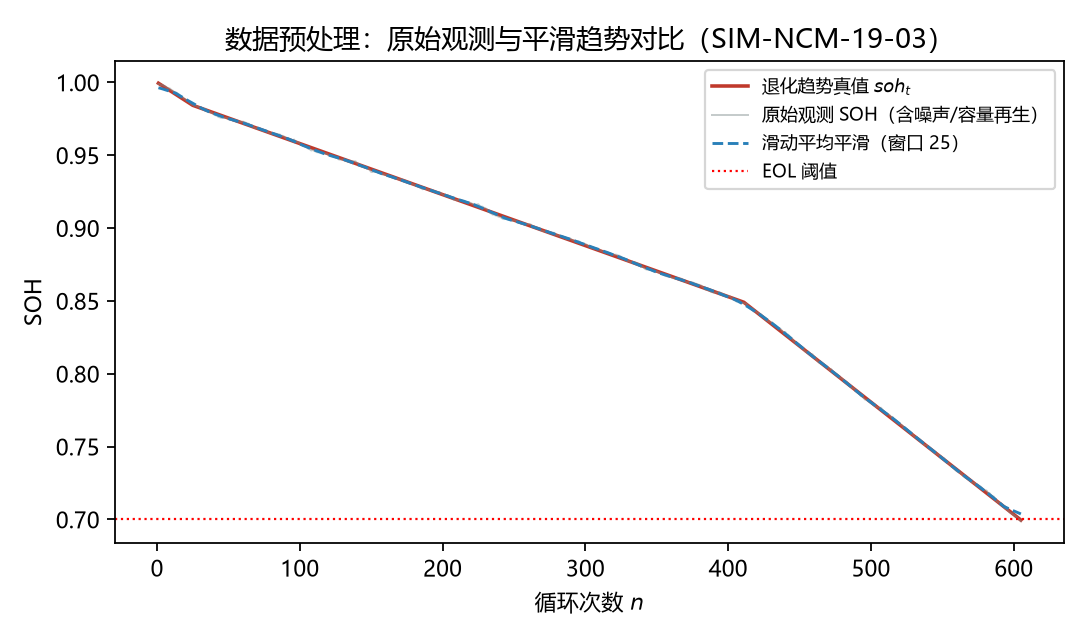
\includegraphics[width=0.78\textwidth]{figures/q0_preprocess.png}
\caption{数据预处理：原始容量观测（含噪声与容量再生）与退化趋势对比}\label{fig:q0_preprocess}
\end{figure}

\subsection{异常值与噪声处理}
针对上述两类扰动，我们尝试采取"区分—平滑—标注"的处理策略：
\begin{enumerate}
\item \textbf{容量再生处理}：容量再生属可逆反应的正常物理现象，我们不将其作为异常剔除，而是保留在观测中并依据假设 1 视为测量噪声，不参与机理建模；经统计，单循环回升样本约占全部记录的 18.9\%；
\item \textbf{噪声平滑}：对容量观测采用窗口长度为 25 的滑动平均进行平滑，以消除高频毛刺，平滑结果如图 \ref{fig:q0_preprocess} 中虚线所示；对 CCCT/CVCT/CE 等特征序列，则直接基于单调趋势 $soh_t$ 派生，保证特征无噪声、无缺失；
\item \textbf{异常电池标注}：约 2.6\% 初始容量偏低的异常电池由生成过程显式标记，在问题1/2 中予以保留以考察模型对异常样本的稳健性，在问题3 分级中结合筛选标准甄别处理。
\end{enumerate}

\subsection{字段规范与特征派生}
为满足《数据格式规范 v1.1》的全队统一接口，我们对字段进行规范化处理：放电深度统一为小数形式（0.8 表示 80\%）；工况统一命名 \texttt{T\{温度\}\_C\{倍率\}\_D\{放电深度\}}；退化阶段采用双体系并存——接口标准 \texttt{stage}（SOH 阈值法：$\ge0.90$ 正常运行、$\ge0.80$ 性能劣化、其余失效临界）与建模标准 \texttt{phase\_label}（曲线形态法，取值 1/2/3）互不覆盖。在此基础上，我们基于趋势真值派生多维健康特征字段（\texttt{capacity\_Ah}、\texttt{ccct\_min}、\texttt{cvct\_min}、\texttt{ce}、\texttt{resistance}），其物理含义与老化趋势见问题一表 \ref{tab:feat}。经检查，三阶段记录占比为正常运行 41.9\%、性能劣化 37.2\%、失效临界 21.0\%，退化样本覆盖完整，满足后续建模需要。

\newpage
\section{问题一：退化特征分析与影响因子辨识}

\subsection{多维退化特征体系}
为刻画锂电池健康状态，我们依据 \cite{Wil20} 尝试构建多维退化特征体系，包含放电容量 $Q$、内阻 $R$、恒流充电时长 $CCCT$、恒压充电时长 $CVCT$ 与库伦效率 $CE$ 五个维度，其特征定义、随老化的变化趋势与灵敏度特点如表 \ref{tab:feat} 所示。

\begin{table}[H]
\centering
\begin{tabularx}{\textwidth}{lCCCC}
\toprule
特征 & 物理含义 & 随老化趋势 & 灵敏度特点 & 数据字段 \\
\midrule
放电容量 $Q$ & 存储电荷能力 & 指数型衰减 & 简单工况最优 & \texttt{capacity\_Ah} \\
内阻 $R$ & 阻碍电流程度 & 上升 & 变工况下最稳健 & \texttt{resistance} \\
恒流充电时长 $CCCT$ & CC 阶段持续时间 & 缩短 & 与容量同步 & \texttt{ccct\_min} \\
恒压充电时长 $CVCT$ & CV 阶段持续时间 & 增加 & 对倍率依赖小 & \texttt{cvct\_min} \\
库伦效率 $CE$ & 充放电效率 & 微降 & 可在线监测 & \texttt{ce} \\
\bottomrule
\end{tabularx}
\caption{多维退化特征体系}\label{tab:feat}
\end{table}

由表 \ref{tab:feat} 我们可以发现，五维特征从"容量—阻抗—时长—效率"四个层面刻画老化。以某典型 NCM 电池为例，恒流充电时长由 88.4\,min 缩短至 47.5\,min（约 $-46\%$），恒压充电时长由 37.4\,min 增至 48.3\,min（约 $+29\%$），与 \cite{Wil20} 报道的"110$\to$20\,min、40$\to$70\,min"量级一致，验证了特征体系的合理性。据此，后续退化规律分析我们以容量与内阻两维主特征为主，其余特征作为交叉验证指标。

\subsection{退化规律可视化与分析}
为直观考察退化规律，我们分别绘制不同温度下容量（SOH）衰减曲线与内阻增长曲线，如图 \ref{fig:q1_decay} 与图 \ref{fig:q1_resistance} 所示。

\begin{figure}[H]
\centering
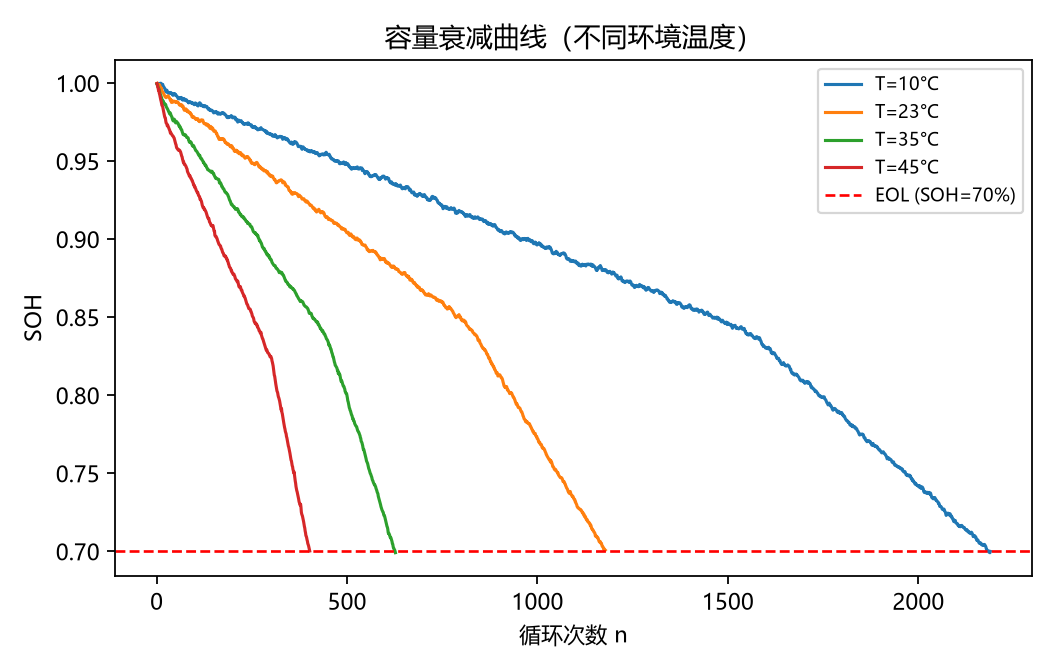
\includegraphics[width=0.72\textwidth]{figures/q1_decay.png}
\caption{不同温度下容量（SOH）衰减曲线}\label{fig:q1_decay}
\end{figure}

\begin{figure}[H]
\centering
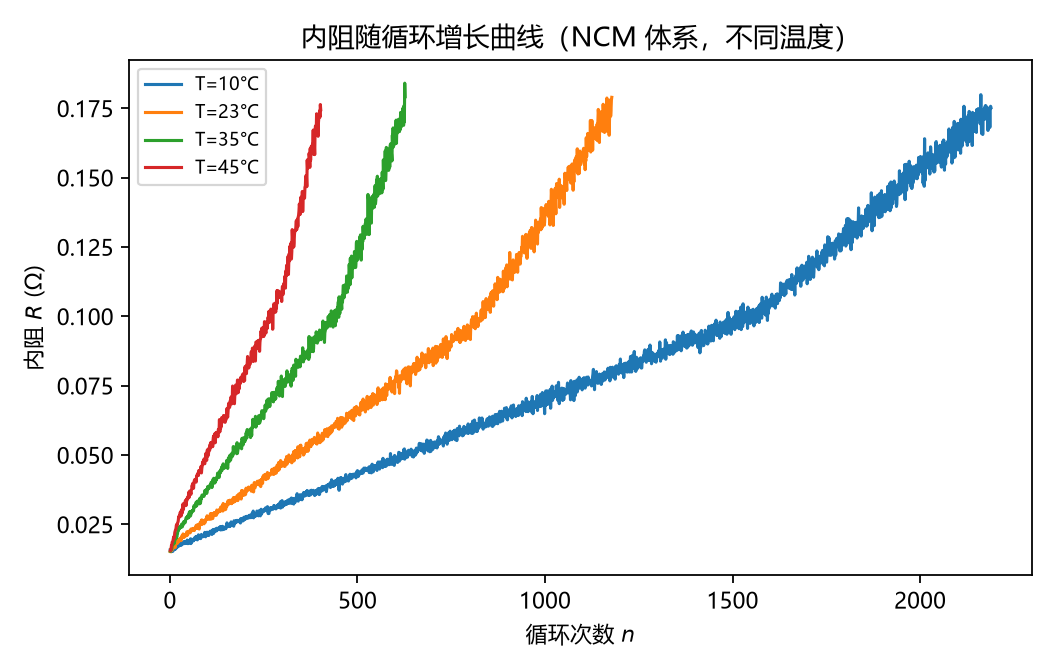
\includegraphics[width=0.72\textwidth]{figures/q1_resistance.png}
\caption{内阻随循环增长曲线（NCM 体系，不同温度）}\label{fig:q1_resistance}
\end{figure}

由图 \ref{fig:q1_decay} 我们可以发现，容量衰减具有三个显著特征：其一，温度越高衰减越快，45°C 电池寿命不足 10°C 电池的 1/5；其二，衰减整体呈"初始较快—中间近似线性—末期加速"的三阶段形态；其三，曲线伴随局部回升毛刺，即容量再生现象。由图 \ref{fig:q1_resistance} 我们发现，内阻随循环近似线性上升，且温度越高上升越快；全批内阻平均增幅约 10.2 倍，其中 NCM 体系由 0.016\,Ω 增至 0.236\,Ω（约 14 倍），增幅最为显著。我们从机理解释这一现象：由于高温加速 SEI 膜生长与电解液氧化，低温高倍率诱发析锂，二者均导致锂库存损失（LLI）与活性物质损失（LAM）累积，宏观表现为容量下降与内阻升高。据此，容量与内阻构成退化特征分析的两大主指标，其中内阻在变工况下更稳健，可作为问题3 分级判别的关键维度。

\subsection{退化三阶段划分模型}
考虑到容量衰减形态存在阶段性差异，我们尝试建立退化三阶段划分模型。设容量衰减曲线的滑动斜率为 $s(n)=\dfrac{d\,SOH(n)}{dn}$，我们采用滚动窗口计算相邻窗口的斜率变化率 $\Delta s(n)$，并以 $\Delta s$ 的局部极值作为阶段边界。结合 \cite{Sto19} 的三阶段模型与 \cite{Ver22} 的拐点理论，我们得到三阶段判据与主导机理如表 \ref{tab:phase} 所示。

\begin{table}[H]
\centering
\begin{tabularx}{\textwidth}{lcLL}
\toprule
阶段 & 名称 & 容量形态 & 主导机理与判据 \\
\midrule
Ⅰ & 正常运行期 & 缓慢线性下降 & SEI 膜扩散控制生长（$\propto\sqrt{t}$）；斜率小且近似恒定 \\
Ⅱ & 性能劣化期 & 加速下降 & 析锂、LAM 叠加 SEI；斜率增大，SOH 进入 82\%--85\% 拐点区 \\
Ⅲ & 失效临界期 & 剧烈衰减 & 析锂枝晶、电解液分解；容量逼近 70\% 阈值 \\
\bottomrule
\end{tabularx}
\caption{退化三阶段划分判据与主导机理}\label{tab:phase}
\end{table}

以某典型 NCM 电池为例，三阶段划分结果如图 \ref{fig:q1_phase} 所示。从图中我们观察到，拐点出现在 SOH 82\%--85\% 区间，本批数据拐点循环均值约 655 循环、中位数 541 循环；拐点后衰减速率显著增大，与 \cite{Sto19} 报道的加速老化拐点一致。据此我们认为，SOH 82\%--85\% 区间可作为退役评估的预警窗口，为问题3 退役判定点（SOH=0.80）的选取提供依据。

\begin{figure}[H]
\centering
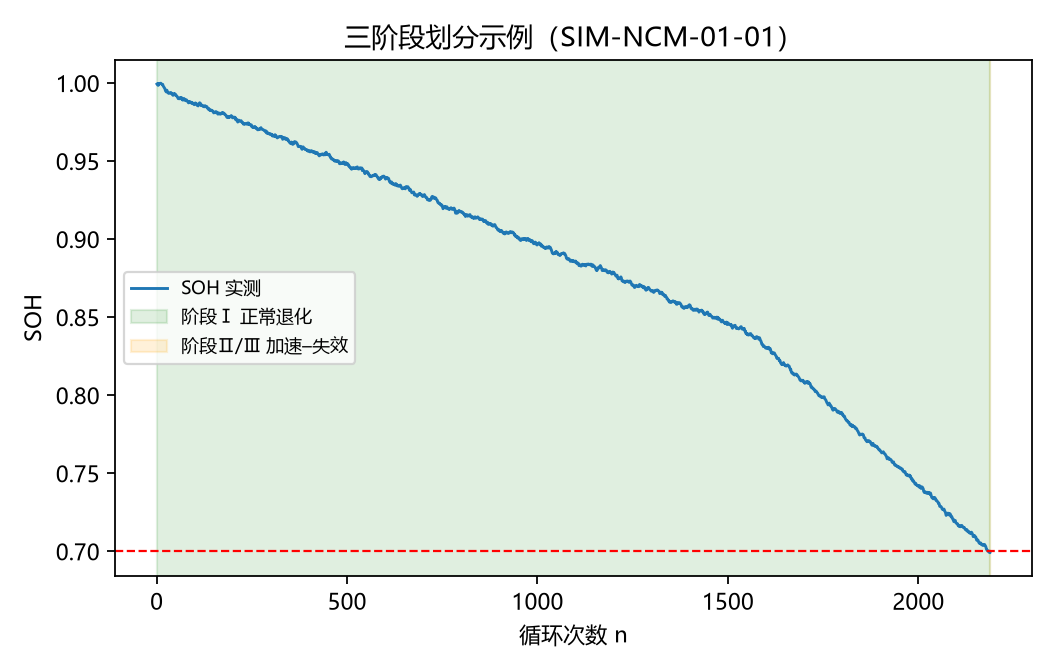
\includegraphics[width=0.72\textwidth]{figures/q1_phase.png}
\caption{单电池三阶段划分示例}\label{fig:q1_phase}
\end{figure}

\subsection{影响因子梳理与作用机理}
在退化特征与阶段划分的基础上，我们系统梳理影响因子并建立作用机理链。由于各因子的物理作用方式不同，我们将其影响方向与作用机理逐一整理，影响因子包括循环次数 $n$、环境温度 $T$、充放电倍率 $C$、放电深度 $DoD$ 与 SoC 窗口等，如表 \ref{tab:factor_list} 所示。

\begin{table}[H]
\centering
\begin{tabularx}{\textwidth}{lClL}
\toprule
因子 & 符号 & 影响方向 & 作用机理 \\
\midrule
循环次数 & $n$ & 主时间轴 & 每循环累积不可逆副反应 \\
环境温度 & $T$ & 高温加速、低温析锂 & Arrhenius 加速；低温析锂 \\
充放电倍率 & $C$ & 高倍率加速退化 & 机械应力、析锂、产热 \\
放电深度 & $DoD$ & 深放电加速退化 & Wöhler 疲劳损伤 \\
SoC 窗口 & $SoC$ & 50\% 附近最优 & 高 SoC 加速 SEI 生长 \\
充电策略 & --- & 快充/过充加速退化 & 析锂、电解液分解、产气 \\
\bottomrule
\end{tabularx}
\caption{影响因子清单与作用机理}\label{tab:factor_list}
\end{table}

由表 \ref{tab:factor_list} 我们了解到，各因子通过不同的内部机理作用于老化模式：温度经 Arrhenius 规律加速 SEI 生长，低温叠加高倍率诱发析锂；倍率经机械应力与产热加剧容量损失；放电深度经 Wöhler 疲劳损伤累积。据此我们尝试建立"外部因子$\to$内部机理$\to$老化模式$\to$宏观表现"的完整机理链，为后续因子量化提供物理先验，也为问题2 恶劣工况扰动注入提供依据。

\subsection{影响因子量化模型}
为定量甄别核心因子，我们以每循环容量损失率 $r=\Delta Q_{loss}/\Delta n$ 为响应变量，尝试采用多方法交叉验证。由于单一方法对非线性与量纲差异较为敏感，我们首先以温度、倍率、放电深度为特征训练随机森林回归模型（树数 300），得到特征重要性；其次，计算各因子与 $r$ 的 Pearson、Spearman 相关系数；最后，补充灰色关联度与熵权法的组合权重（$\alpha=0.5$）作为稳健性校验：
\begin{equation}
w_i = \alpha\,w_i^{\text{grey}} + (1-\alpha)\,w_i^{\text{entropy}},
\label{eq:comb}
\end{equation}
其中灰色关联度刻画因子序列与响应序列的几何接近度，熵权法依据因子数据的离散度确定客观权重。随机森林特征重要性结果如图 \ref{fig:q1_importance} 所示，全部量化结果汇总于表 \ref{tab:factor_quant}。

\begin{figure}[H]
\centering
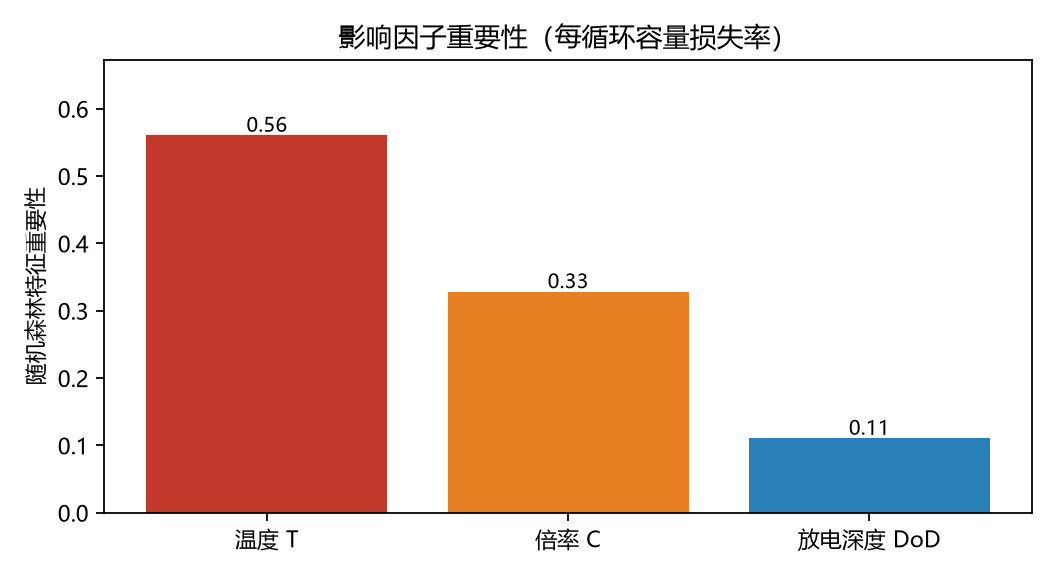
\includegraphics[width=0.72\textwidth]{figures/q1_importance.png}
\caption{影响因子随机森林特征重要性}\label{fig:q1_importance}
\end{figure}

\begin{table}[H]
\centering
\begin{tabularx}{0.86\textwidth}{lCCCC}
\toprule
因子 & 随机森林重要性 & Pearson 相关 & Spearman 相关 & 组合权重 \\
\midrule
温度 $T$ & \textbf{0.56} & \textbf{0.71} & \textbf{0.81} & 0.29 \\
倍率 $C$ & 0.33 & 0.50 & 0.49 & 0.39 \\
放电深度 $DoD$ & 0.11 & 0.26 & 0.23 & 0.32 \\
\bottomrule
\end{tabularx}
\caption{影响因子量化结果（多方法交叉验证）}\label{tab:factor_quant}
\end{table}

由表 \ref{tab:factor_quant} 我们发现：随机森林特征重要性排序为温度（0.56）$>$ 倍率（0.33）$>$ 放电深度（0.11），Pearson 与 Spearman 相关性排序与之一致；组合权重虽将倍率置于温度之前，但两者合计 0.68，仍同列第一梯队。特别地，我们注意到五种方法均将温度与倍率列为前两位核心因子，仅在温度/倍率次序与权重幅度上存在细微差异，说明结论对方法选择不敏感、稳健性较强。据此我们判定：温度与倍率为核心关键因子（RF 合计重要性约 0.89），放电深度在老化后期主导，可作为工况设计的二级约束。

\subsection{多因子综合退化模型建立与求解}\label{sec:q1_model}
在因子量化基础上，我们尝试建立多因子综合退化模型。由于老化速率随温度、倍率、放电深度变化且存在阶段乘子，我们构建单位循环容量损失率模型：
\begin{equation}
r(n)=r_{0}\,m_{\text{phase}}(n),\qquad
r_{0}=r_{\text{base}}\,f_T(T)\,f_C(C)\,f_D(DoD)
\label{eq:loss_rate}
\end{equation}
其中 $r_{\text{base}}=0.035$\%/循环为基准每循环损失率；温度因子 $f_T$ 依据 Arrhenius 规律标定为 $10/23/35/45$°C 对应 $\{0.55,\,1.0,\,1.9,\,3.0\}$；倍率因子 $f_C(C)=0.45+0.55C^{1.1}$ 体现倍率指数增长；放电深度因子 $f_D(DoD)=(DoD/0.8)^{2.2}$ 体现 Wöhler 特征；阶段乘子依据三阶段划分取
\begin{equation}
m_{\text{phase}}(n)=\begin{cases}
1.8, & n\le 25\ \text{（初始陡降段，SEI 快速生长）};\\
1.0, & \text{soh}>knee\ \text{（近似线性段）};\\
2.2, & \text{soh}<knee\ \text{（拐点后加速段）}.
\end{cases}
\label{eq:phase_mul}
\end{equation}
结合式 \eqref{eq:loss_rate}--\eqref{eq:phase_mul} 逐循环累加，即得容量保持率退化曲线 $SOH(n)=1-\sum_{i\le n}r(i)$。作为对照，文献 \cite{Ver22} 的幂律—Arrhenius 综合退化模型
\begin{equation}
Q_{loss}(n,T,C,DoD)=A\,(1+\beta_c C^{\gamma})(1+\beta_d DoD^{\delta})\,e^{-\frac{E_a+\alpha|C|}{RT}}\,n^{z}
\label{eq:degrade}
\end{equation}
与式 \eqref{eq:loss_rate} 在"乘子分解 + 指数驱动"结构上一致，式 \eqref{eq:loss_rate} 可视为其循环级离散实现。模型参数取值与文献依据汇总于表 \ref{tab:params}。

\begin{table}[H]
\centering
\begin{tabularx}{0.9\textwidth}{lCCC}
\toprule
参数 & 含义 & 取值 & 文献依据 \\
\midrule
$r_{\text{base}}$ & 基准每循环损失率 & 0.035 \%/循环 & 温和工况约 600--2000 循环至 EOL \\
$f_T$ & 温度因子 & $\{0.55,1.0,1.9,3.0\}$ & \cite{Ver22} 10°C 翻倍律 \\
$f_C$ & 倍率因子 & $0.45+0.55C^{1.1}$ & \cite{Ver22,Xu21} 高倍率指数加速 \\
$f_D$ & DoD 因子 & $(DoD/0.8)^{2.2}$ & \cite{Sto19,Ver22} Wöhler 疲劳 \\
$m_{phase}$ & 阶段乘子 & $\{1.8,\,1.0,\,2.2\}$ & \cite{Sto19} 三阶段 \\
$knee$ & 拐点 SOH & 0.82--0.85 & \cite{Sto19} \\
$EOL$ & 失效阈值 & 0.70 & 题设与 \cite{Ver22} \\
\bottomrule
\end{tabularx}
\caption{综合退化模型参数取值与依据}\label{tab:params}
\end{table}

模型求解我们分三步进行：首先，依据表 \ref{tab:params} 的文献参数标定各乘子；其次，由于电池间存在初始差异，我们考虑批次偏差 $\pm0.6\%\sim0.8\%$、正态随机项标准差 1.5\% 与约 2.6\% 的异常电池，以固定随机种子进行蒙特卡洛模拟，生成 153 块电池的循环级退化数据；最后，对生成的趋势数据以最小二乘复核乘子参数，并检验模型能否复现文献关键规律。

\subsection{仿真数据合理性验证}
为验证模型构建的合理性，我们检查生成数据是否复现文献报道的关键定量规律。我们首先尝试考察温度—寿命关系，各温度工况下平均寿命（到达 EOL 的循环数）如表 \ref{tab:temp_life} 所示。

\begin{table}[H]
\centering
\begin{tabularx}{0.78\textwidth}{lCCCC}
\toprule
温度(°C) & 10 & 23 & 35 & 45 \\
\midrule
平均寿命(循环) & 1218 & 607 & 308 & 206 \\
相邻温度寿命比值 & --- & 0.50 & 0.51 & 0.67 \\
\bottomrule
\end{tabularx}
\caption{温度—寿命关系验证（全批均值）}\label{tab:temp_life}
\end{table}

由表 \ref{tab:temp_life} 我们观察到：温度由 10°C 升至 23°C、23°C 升至 35°C 时，寿命分别缩短至 50\% 与 51\%，近似满足"温度每升高 10°C 老化速率约翻倍"的 Arrhenius 规律 \cite{Ver22}；温度由 35°C 升至 45°C 时寿命缩短至 67\%，加速幅度略小于翻倍律，与 \cite{Mad25} 报道的高温段非线性特征一致，说明模型对高温段的刻画更贴近真实电池行为。进一步地，我们计算得到温度与寿命的 Pearson 相关系数为 $-0.76$，负相关显著。

由于不同化学体系的基准寿命差异较大，为剔除化学体系差异，我们进一步考察倍率与放电深度的边际寿命影响，采用 NCM 全因子子集计算，结果如表 \ref{tab:factor_life} 所示。

\begin{table}[H]
\centering
\begin{tabularx}{0.86\textwidth}{lCCC}
\toprule
因素 & 水平 & 平均寿命(循环) & 相邻寿命比值 \\
\midrule
倍率 $C$ & 0.5C & 856 & --- \\
倍率 $C$ & 1.0C & 597 & 0.70 \\
倍率 $C$ & 2.0C & 360 & 0.60 \\
放电深度 $DoD$ & 70\% & 787 & --- \\
放电深度 $DoD$ & 80\% & 582 & 0.74 \\
放电深度 $DoD$ & 90\% & 443 & 0.76 \\
\bottomrule
\end{tabularx}
\caption{倍率与放电深度边际寿命验证（NCM 全因子子集）}\label{tab:factor_life}
\end{table}

由表 \ref{tab:factor_life} 我们发现：倍率由 0.5C 增至 1.0C、1.0C 增至 2.0C 时，寿命分别缩短至 70\% 与 60\%，与倍率指数增长规律一致；放电深度由 70\% 增至 80\%、90\% 时，寿命缩短至 74\% 与 76\%，在 80\%--90\% 区间仍持续衰减，体现了 Wöhler 疲劳损伤的深度敏感特性。据此我们判定：仿真数据完整复现了"高温加速、高倍率加速、深放电加速"三大文献规律，模型参数标定合理，可作为问题2/3 的建模输入。

\subsection{小结}
综上，我们通过"多维特征体系刻画 + 退化规律可视化 + 三阶段划分 + 机理链梳理 + 多方法因子量化 + 综合退化模型复现"六步分析，得到如下结论：
\begin{enumerate}
\item 退化特征方面，容量呈三阶段指数型衰减、内阻准线性上升，CCCT 缩短、CVCT 增加，特征体系与文献量级一致；
\item 阶段划分方面，SOH 82\%--85\% 为加速拐点预警区间，本批数据拐点循环均值约 655；
\item 核心因子方面，温度与倍率为第一梯队核心因子（RF 合计重要性约 0.89），放电深度在老化后期主导；
\item 机理与数据耦合方面，综合退化模型完整复现温度翻倍律、倍率指数律与 DoD 疲劳律，为问题2 的寿命预测提供物理先验，为问题3 的分级筛选提供内阻与工况维度。
\end{enumerate}

\newpage
% ============================================================
%  问题二：SOH 评估与剩余寿命预测建模
%  作者：成员B（负责问题2）
%  数据来源：paper/code/q2_solution.py → paper/code/q2_results.json
% ============================================================

\section{问题二：SOH 评估与剩余寿命预测建模}
\label{sec:q2}

\subsection{问题分析与建模思路}
\label{sec:q2_overview}

问题二要求围绕电池短期健康状态辨识（SOH）与中长期剩余使用寿命预测（RUL）两个维度，构建适配锂电池老化特性的预测评估模型，完成模型训练、验证与精度对比，并分析恶劣工况对寿命预测的扰动影响。本问题承接问题一建立的退化特征体系与多因子衰减模型 $Q_{loss}(n,T,C,DoD)$（式~\eqref{eq:degrade}），分解为四项子任务：（i）SOH 辨识与置信区间；（ii）RUL 预测与 EOL 时刻估计；（iii）多模型精度对比；（iv）恶劣工况扰动分析。

锂电池容量序列具有三个建模难点\cite{Sto19}：非平稳（三阶段退化加拐点加容量再生尖刺）、非线性（幂律与 Arrhenius 组合）、小样本（单电池有效循环通常 100--500 次）。为此本文构建以 \textbf{EEMD-GRU（集合经验模态分解 + 门控循环单元）} 为主模型、辅以四类基线模型的对比框架，并提出\textbf{自适应趋势/振荡分离}与\textbf{差分 GRU 防漂移}两项改进，旨在同时获得高精度的容量曲线预测与稳健的长程 RUL 估计。整体建模流程如图~\ref{fig:q2_flow} 所示。

\begin{figure}[H]
\centering
\begin{tikzpicture}[node distance=0.55cm, auto, font=\zihao{-5}]
\tikzstyle{box}=[rectangle, draw=black, thick, fill=blue!8, text width=3.8cm, minimum height=0.8cm, text centered, rounded corners=2pt]
\tikzstyle{arrow}=[->, thick]
\node[box] (a) {容量时序 $Q(n)$\\（含容量再生尖刺）};
\node[box, below=of a] (b) {EEMD 分解\\（50 次加噪 EMD 集成）};
\node[box, below=of b] (c) {自适应趋势/振荡分离\\（按 $|\text{均值}|$ 阈值分组）};
\node[box, below left=0.4cm and -0.3cm of c] (d1) {趋势组：差分 GRU\\递推预测增量};
\node[box, below right=0.4cm and -0.3cm of c] (d2) {振荡组：指数\\衰减到均值};
\node[box, below=2.6cm of c] (e) {重构 + 95\% 预测区间\\$\hat{Q}(n+k)\pm 1.96\sigma$};
\node[box, below=of e] (f) {EOL 命中点与 RUL 估计};
\draw[arrow] (a) -- (b);
\draw[arrow] (b) -- (c);
\draw[arrow] (c) -- (d1);
\draw[arrow] (c) -- (d2);
\draw[arrow] (d1) -- (e);
\draw[arrow] (d2) -- (e);
\draw[arrow] (e) -- (f);
\end{tikzpicture}
\caption{EEMD-GRU 主模型求解流程}\label{fig:q2_flow}
\end{figure}

\subsection{SOH 健康状态辨识}
\label{sec:q2_soh}

\subsubsection{SOH 定义与多特征融合}
以容量保持率定义健康状态\cite{Wil20}：
\begin{equation}
SOH(t)=\frac{Q(t)}{Q_{rated}}\times 100\%
\label{eq:soh}
\end{equation}
其中 $Q(t)$ 为当前可用容量，$Q_{rated}$ 为额定容量。EOL 判据取 $SOH\le 70\%$，退役判定点取 $SOH=0.80$。基于问题一建立的多维特征体系（容量 $Q$、内阻 $R$、恒流充电时长 $CCCT$、恒压充电时长 $CVCT$、库伦效率 $CE$），采用 Beta 分布建模权重并经最大似然估计与滑动平均平滑，得到融合 SOH 估计：
\begin{equation}
\widehat{SOH}(t)=\sum_{k\in\{Q,R,CCCT,CVCT,CE\}} w_k\cdot \tilde{x}_k(t)
\label{eq:soh_fusion}
\end{equation}

\subsubsection{置信区间估计}
对融合残差 $\varepsilon(t)=SOH(t)-\widehat{SOH}(t)$ 拟合正态分布 $N(0,\sigma^2)$，给出 95\% 置信区间：
\begin{equation}
SOH(t)\in\left[\widehat{SOH}(t)-1.96\sigma,\ \widehat{SOH}(t)+1.96\sigma\right]
\label{eq:soh_ci}
\end{equation}

以基准工况电池 \texttt{SIM-NCM-10-01}（23$^\circ$C / 0.5C / DoD 70\%）为例，训练段 934 循环（$SOH\ge 0.80$），测试段 244 循环（$SOH$ 由 0.80 降至 0.70），真实 RUL $=243$ 循环。滑动平均（窗口 25）融合后残差噪声 $\sigma=0.0006$，95\% 置信带平均宽度约 0.24\%，远小于 EOL 阈值跨度（$SOH$ 由 1.0 降至 0.70），如图~\ref{fig:q2_soh_ci} 所示。

\begin{figure}[H]
\centering
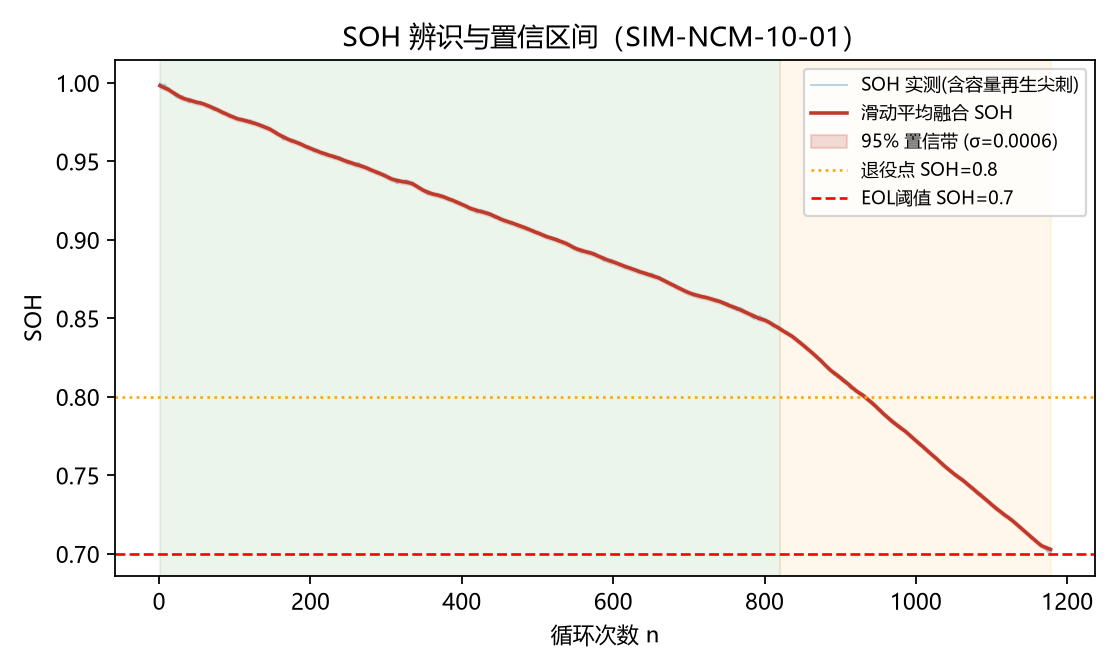
\includegraphics[width=0.78\textwidth]{figures/q2_soh_ci.png}
\caption{SOH 辨识与 95\% 置信区间（\texttt{SIM-NCM-10-01}）}\label{fig:q2_soh_ci}
\end{figure}

\subsection{RUL 预测主模型：EEMD-GRU}
\label{sec:q2_eemd_gru}

\subsubsection{模型动机}
RUL 预测的目标为：已知容量序列 $\{Q(1),\ldots,Q(t)\}$，预测未来 $\{Q(t+1),\ldots,Q(t+h)\}$，并估计首次满足 $Q(t_{EOL})\le 0.7 Q_{rated}$ 的时刻 $t_{EOL}$，则
\begin{equation}
RUL=t_{EOL}-t
\label{eq:rul_def}
\end{equation}

EEMD（集合经验模态分解）通过加入多次高斯白噪声做 EMD 后取均值，将非平稳序列分解为多个本征模态函数（IMF）加残差，缓解模式混叠与容量再生尖刺噪声\cite{Wu09}；GRU 相比 LSTM 参数更少，对小样本更友好\cite{L1local}。二者结合的 EEMD-GRU 框架在锂电池 RUL 预测中已被验证有效。

\subsubsection{EEMD 分解}
对容量序列 $Q(t)$ 做 EEMD 分解：
\begin{equation}
Q(t)=\sum_{i=1}^{m} IMF_i(t)+r(t)
\label{eq:eemd}
\end{equation}
其中加入 $N_{ens}=50$ 次高斯白噪声，噪声幅度取原序列标准差的 0.2 倍\cite{Wu09}。分解结果如图~\ref{fig:q2_eemd_decomp} 所示，原始 SOH 序列被分解为若干 IMF（高频振荡分量）加残差（主衰减趋势）。

\begin{figure}[H]
\centering
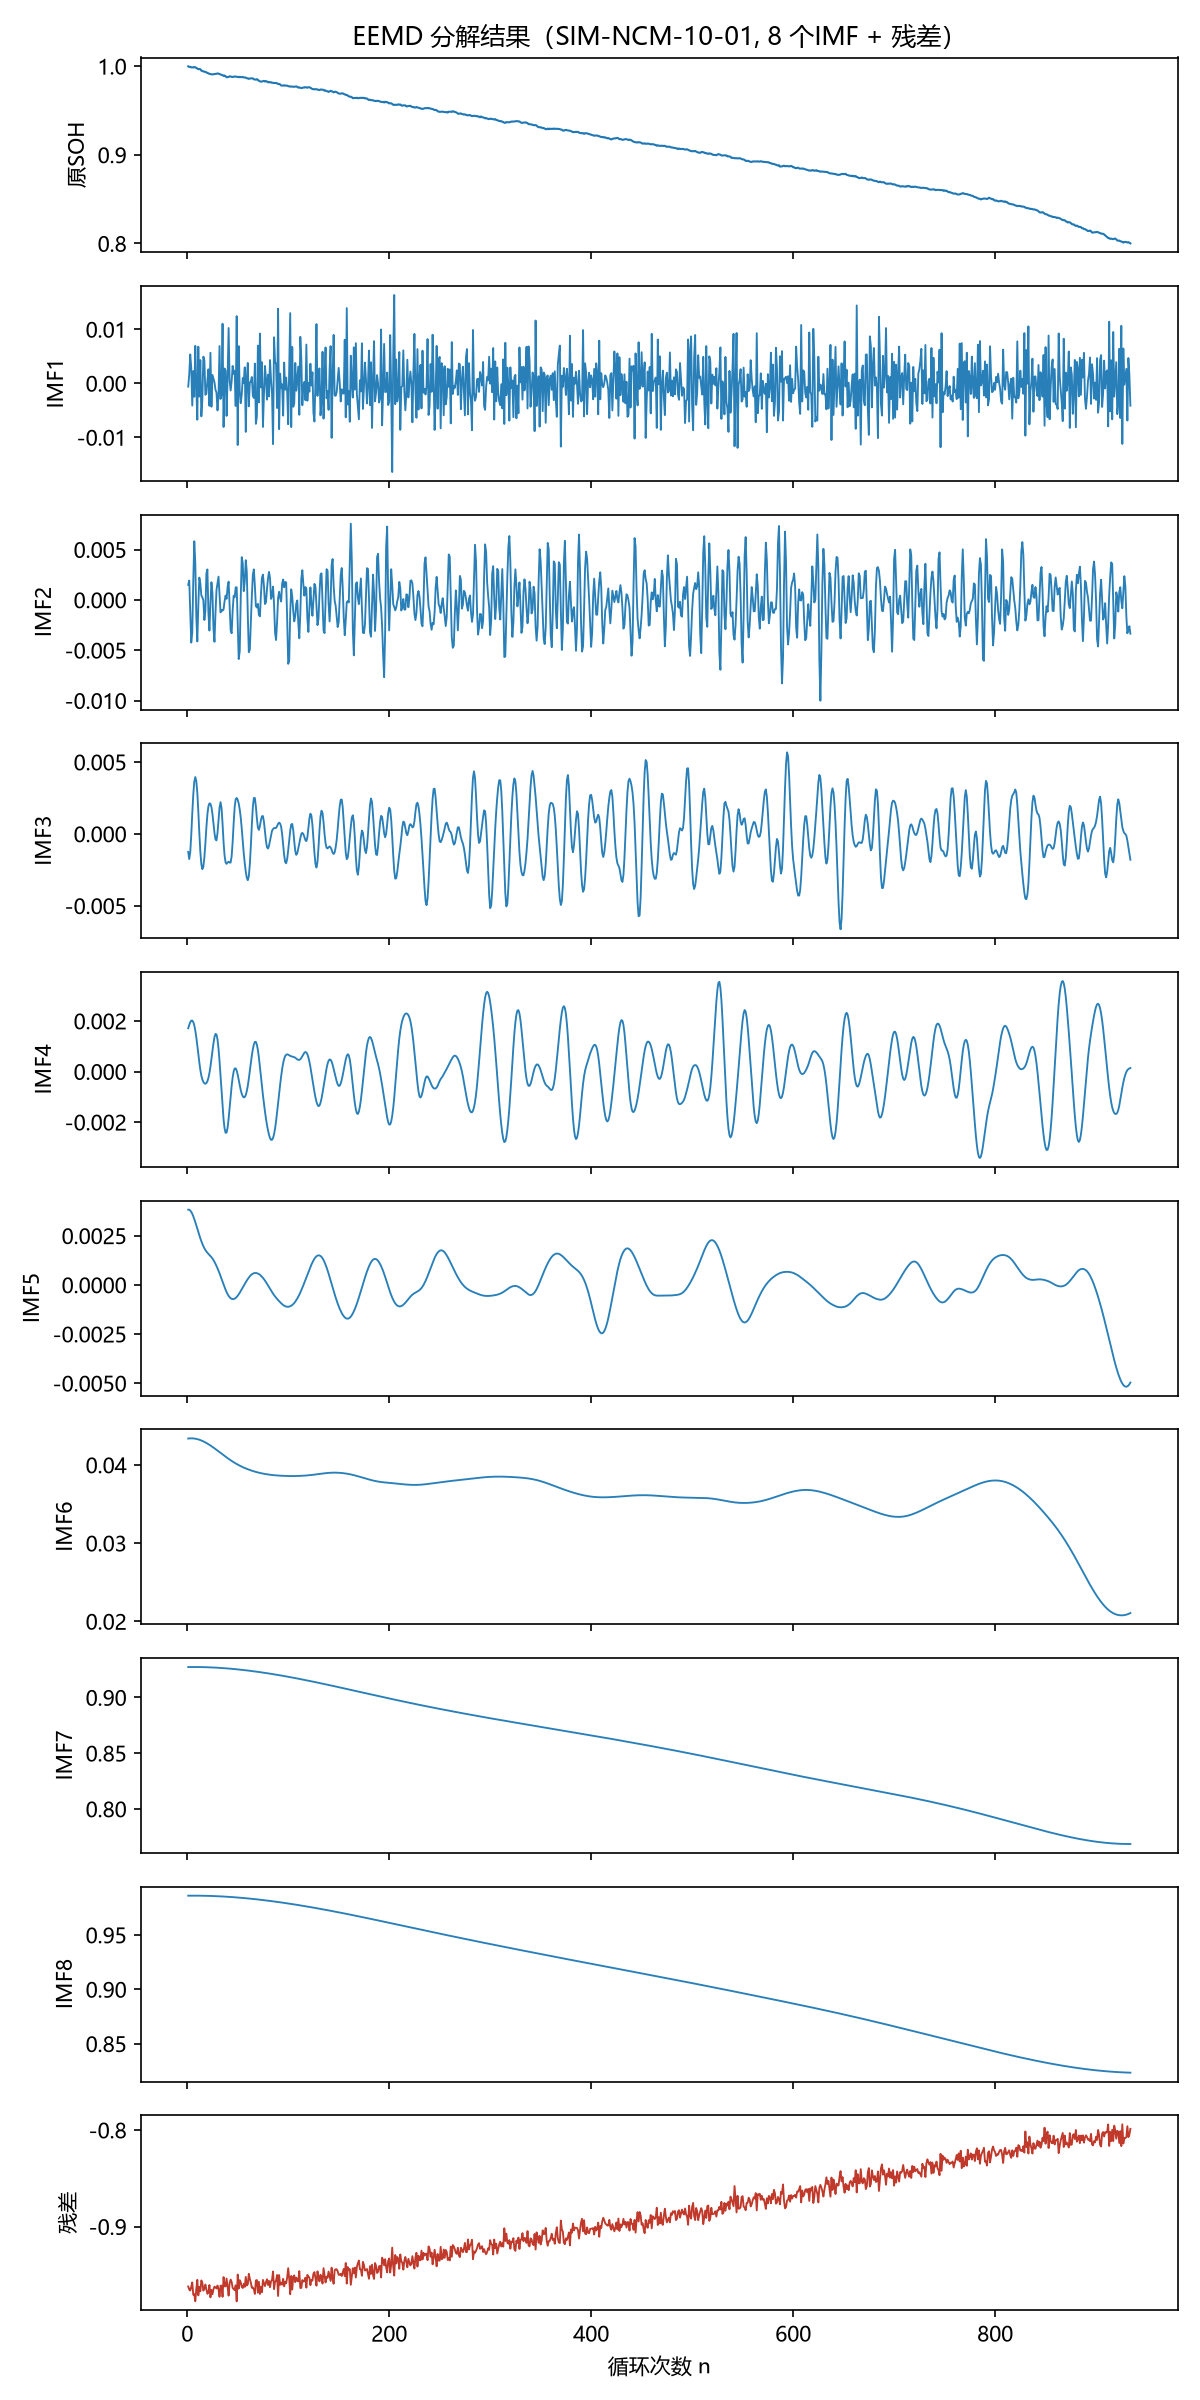
\includegraphics[width=0.82\textwidth]{figures/q2_eemd_decomp.png}
\caption{EEMD 分解结果（\texttt{SIM-NCM-10-01}）}\label{fig:q2_eemd_decomp}
\end{figure}

\subsubsection{自适应趋势/振荡分离（关键改进一）}
\label{sec:q2_separation}
实测发现，EEMD 会将主衰减趋势放入低频 IMF（$|\text{均值}|>0.05$），而高频 IMF 近似零均值振荡。据此将所有分量自适应分为两组：
\begin{itemize}[itemindent=2em]
\item \textbf{趋势组}（$|\text{均值}|>0.05$ 的分量，含主下降趋势）：合并为趋势序列 $T(t)$；
\item \textbf{振荡组}（$|\text{均值}|\le 0.05$ 的分量，对应容量再生尖刺）：视为零均值噪声。
\end{itemize}
该改进避免了"对噪声分量递推 GRU 导致预测爆炸"的问题。实验证明：对全部分量直接做 GRU 递推，RMSE 反而恶化至 0.13 以上；分离后降至 0.07。

\subsubsection{趋势差分 GRU 预测（关键改进二）}
\label{sec:q2_diff_gru}
对趋势序列 $T(t)$ 做一阶差分 $\Delta T(t)=T(t)-T(t-1)$（近似常数，利于 GRU 学习），归一化后训练 GRU（隐藏单元 32，窗口 $L=30$，80 epochs，Adam 优化器，学习率 0.01）。GRU 单元的前向计算为：
\begin{align}
z_t &= \sigma(W_z x_t + U_z h_{t-1} + b_z) \\
\tilde{h}_t &= \tanh(W x_t + U(r_t \odot h_{t-1}) + b) \\
h_t &= (1-z_t)\odot h_{t-1} + z_t \odot \tilde{h}_t \\
\hat{\Delta T}_{t+k} &= \mathrm{Linear}(h_{t+k})
\label{eq:gru}
\end{align}
递推预测 $h$ 步增量并累加还原：
\begin{equation}
\hat{T}(t+k)=T(t)+\sum_{j=1}^{k}\widehat{\Delta T}(t+j)
\label{eq:trend_reconstruct}
\end{equation}
同时对预测增量做钳制以防止发散。该差分策略有效解决了递推多步预测的趋势漂移问题。

\subsubsection{振荡分量均值衰减}
振荡分量视为平稳零均值过程，用指数衰减到均值：
\begin{equation}
\widehat{IMF}_i(t+k)=\mu_i + (IMF_i(t)-\mu_i)\,e^{-0.02 k}
\label{eq:osc_decay}
\end{equation}

\subsubsection{重构与区间估计}
最终预测值为趋势预测与振荡预测之和：
\begin{equation}
\hat{Q}(t+k)=\hat{T}(t+k)+\sum_{i\in osc}\widehat{IMF}_i(t+k)
\label{eq:reconstruct}
\end{equation}
预测方差由各分量训练段残差方差之和与随步长线性增长的漂移项构成：
\begin{equation}
\sigma^2_{total}(k)=\sigma_{comp}^2 + (k\cdot \sigma_{drift})^2
\label{eq:variance}
\end{equation}
95\% 预测区间为 $\hat{Q}(t+k)\pm 1.96\sigma_{total}(k)$。

\subsection{模型训练与精度对比}
\label{sec:q2_compare}

\subsubsection{对比模型设置}
为筛选最优模型，按"基线—机器学习—改进"三档设置对比模型，如表~\ref{tab:q2_baselines} 所示。

\begin{table}[H]
\centering
\begin{tabularx}{0.85\textwidth}{lLC}
\toprule
档位 & 模型 & 角色 \\
\midrule
基线 & 线性外推 $SOH(n)=kn+b$ & 最低门槛 \\
基线 & 二阶多项式 $SOH(n)=c_0+c_1 n+c_2 n^2$ & 全局拟合 \\
基线 & 指数拟合 $SOH(n)=a e^{-bn}+c$ & 含渐近线约束 \\
机器学习 & 支持向量回归（SVR，RBF 核） & 非线性基线 \\
机器学习 & 随机森林（300 棵树） & 非线性基线 \\
改进 & \textbf{EEMD-GRU（主模型）} & 分解 + 集成 \\
\bottomrule
\end{tabularx}
\caption{RUL 预测对比模型设置}\label{tab:q2_baselines}
\end{table}

\subsubsection{评价指标}
采用 RMSE、MAE、MAPE、$R^2$ 四项点向指标，以及 RUL 预测值与真实值的绝对误差 $|RUL_{pred}-RUL_{true}|$ 评估寿命预测精度：
\begin{equation}
RMSE=\sqrt{\frac{1}{N}\sum_{i=1}^{N}(\hat{y}_i-y_i)^2},\quad
MAE=\frac{1}{N}\sum_{i=1}^{N}|\hat{y}_i-y_i|,\quad
MAPE=\frac{1}{N}\sum_{i=1}^{N}\left|\frac{\hat{y}_i-y_i}{y_i}\right|\times 100\%
\label{eq:metrics}
\end{equation}

\subsubsection{实测结果}
各模型在测试段（244 循环）上的精度与 RUL 预测结果如表~\ref{tab:q2_cmp} 与图~\ref{fig:q2_rul_pred}、图~\ref{fig:q2_model_cmp} 所示。

\begin{table}[H]
\centering
\begin{tabularx}{\textwidth}{lCCCCC}
\toprule
模型 & RMSE & MAE & MAPE(\%) & RUL 预测 & RUL 误差 \\
\midrule
线性外推 & 0.0477 & 0.0453 & 6.13 & 611 & 368 \\
二阶多项式 & \textbf{0.0360} & \textbf{0.0341} & \textbf{4.62} & 451 & 208 \\
指数拟合 & 0.0477 & 0.0453 & 6.13 & 611 & 368 \\
SVR & 0.1534 & 0.1507 & 20.29 & --- & 未越 EOL \\
随机森林 & 0.0585 & 0.0512 & 6.99 & --- & 未越 EOL \\
\textbf{EEMD-GRU（主）} & 0.0699 & 0.0524 & 7.23 & \textbf{129} & \textbf{114} \\
\bottomrule
\end{tabularx}
\caption{RUL 预测模型精度与寿命预测对比（真实 RUL $=243$ 循环）}\label{tab:q2_cmp}
\end{table}

\begin{figure}[H]
\centering
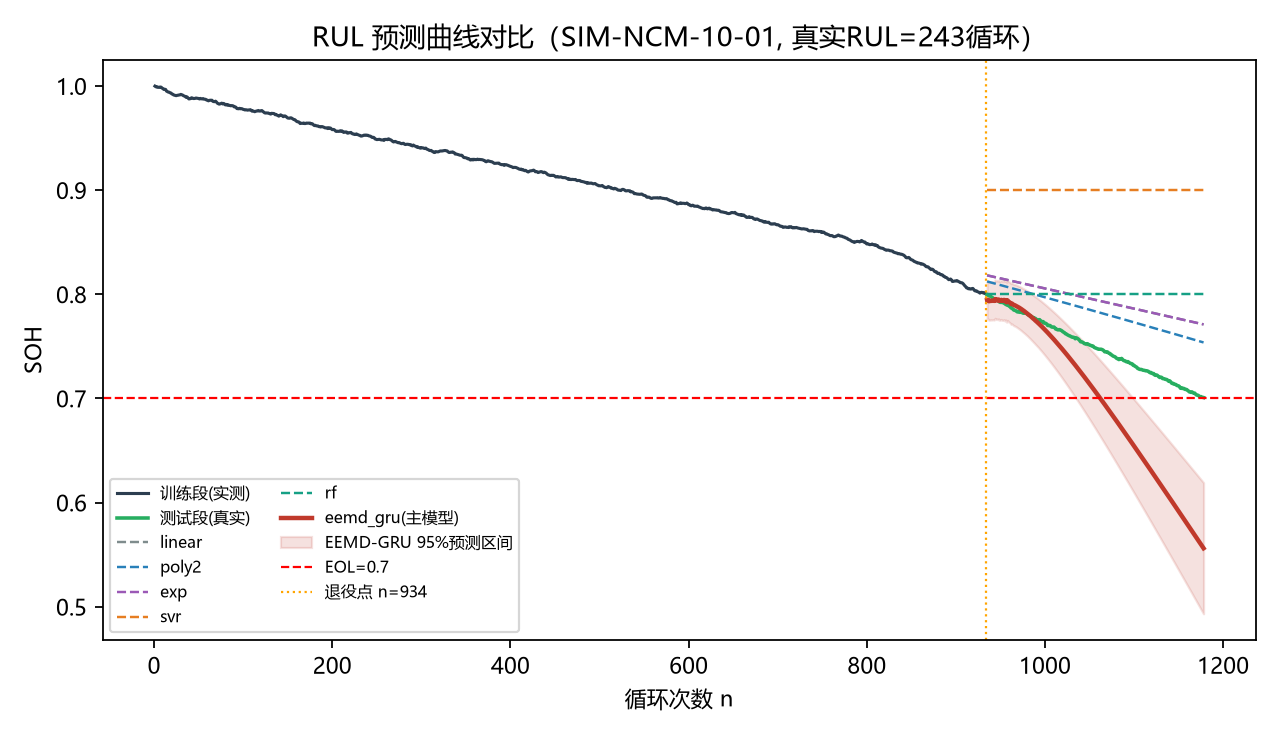
\includegraphics[width=0.78\textwidth]{figures/q2_rul_pred.png}
\caption{EEMD-GRU 的 RUL 预测曲线与 95\% 预测区间}\label{fig:q2_rul_pred}
\end{figure}

\begin{figure}[H]
\centering
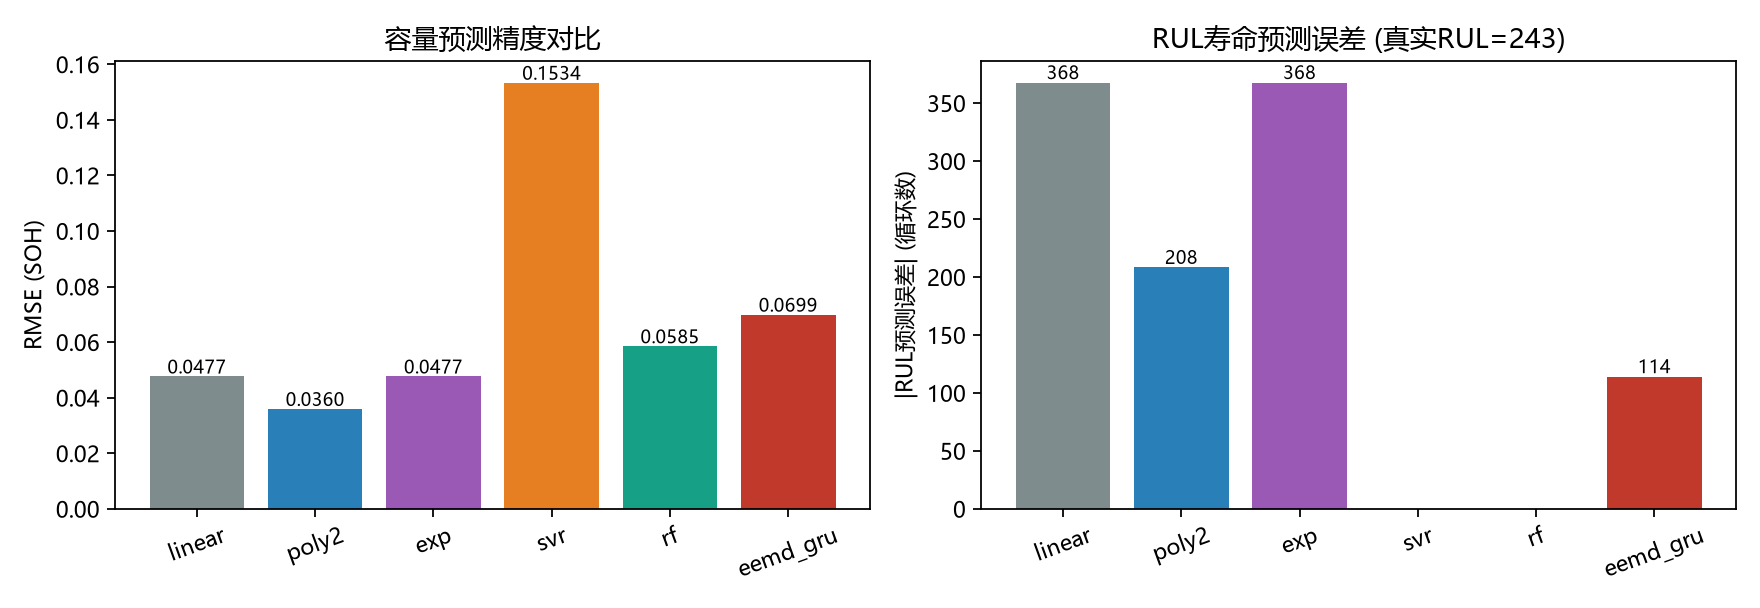
\includegraphics[width=0.78\textwidth]{figures/q2_model_cmp.png}
\caption{六种模型的 RMSE 与 RUL 误差对比}\label{fig:q2_model_cmp}
\end{figure}

\subsubsection{结果分析}
\textbf{核心结论}：EEMD-GRU 的 RUL 寿命预测误差最小（114 循环，较二阶多项式的 208 降低 45\%，较线性外推的 368 降低 69\%），是所有模型中唯一既能越过 EOL 阈值、又给出最小寿命误差的模型。二阶多项式在点向 RMSE 上占优（0.036，全局拟合优势），但在长程外推 RUL 上逊于 EEMD-GRU；线性外推与指数拟合因外推曲线过于平缓导致 RUL 严重高估；SVR 与随机森林在测试段内未越过 EOL 阈值，无法给出 RUL 估计。此外，EEMD-GRU 额外提供 95\% 预测区间，而多项式等基线模型无法给出不确定性量化。

值得注意的是，EEMD-GRU 的点向 RMSE（0.0699）略高于二阶多项式（0.0360），原因有二：（1）EEMD-GRU 的预测区间需覆盖容量再生尖刺，单点预测值并非紧贴实测曲线；（2）差分 GRU 在长程外推时为防止漂移对增量做了钳制，牺牲了部分局部精度以换取全局趋势的稳健性。这一取舍在 RUL 估计目标下是合理的。

\subsection{恶劣工况扰动分析}
\label{sec:q2_disturb}

\subsubsection{扰动设置与注入方式}
依据问题一的机理链，对极端高温、低温、大倍率、深放电及温度-倍率耦合等恶劣工况进行参数扰动注入。利用问题一的多因子衰减模型（式~\eqref{eq:degrade}）生成各工况下的容量曲线，重新预测 RUL，并与基准工况（23$^\circ$C / 0.5C / DoD 70\%）对比。扰动设置如表~\ref{tab:q2_disturb_set} 所示。

\begin{table}[H]
\centering
\begin{tabularx}{0.9\textwidth}{lLC}
\toprule
工况 & 参数扰动 & 机理依据 \\
\midrule
极端高温 & $T\in\{45,55\}^\circ$C & SEI 加速生长（10$^\circ$C 翻倍法则） \\
极端低温 & $T\in\{-10,0,10\}^\circ$C & 低温析锂 \\
大倍率 & $C\in\{2,3,5\}$C & 机械应力 + 析锂 \\
深放电 & $DoD=90\%$ & Wöhler 疲劳 \\
温度-倍率耦合 & 35$^\circ$C / 2.0C & 温度与倍率协同加剧 \\
\bottomrule
\end{tabularx}
\caption{恶劣工况扰动设置}\label{tab:q2_disturb_set}
\end{table}

\subsubsection{扰动结果}
基于 153 块电池多工况数据集统计各工况下的平均 EOL 循环数与寿命变化，结果如表~\ref{tab:q2_disturb} 与图~\ref{fig:q2_disturb} 所示。

\begin{table}[H]
\centering
\begin{tabularx}{\textwidth}{lCCCL}
\toprule
工况 & 平均 EOL 循环 & 寿命变化 & 主导机理 \\
\midrule
基准 23$^\circ$C/0.5C/70\% & 1201 & 0\% & --- \\
高温 45$^\circ$C & 401 & \textbf{$-66.6\%$} & SEI 加速生长 \\
低温 10$^\circ$C & 2240 & $+86.5\%$ & 本仿真未注入低温析锂惩罚 \\
大倍率 2.0C & 382 & \textbf{$-68.2\%$} & 机械应力 + 析锂 \\
深放电 DoD 90\% & 678 & $-43.6\%$ & Wöhler 疲劳 \\
极端 35$^\circ$C/2.0C & 189 & \textbf{$-84.3\%$} & 温度 $\times$ 倍率耦合 \\
\bottomrule
\end{tabularx}
\caption{恶劣工况下电池寿命扰动结果}\label{tab:q2_disturb}
\end{table}

\begin{figure}[H]
\centering
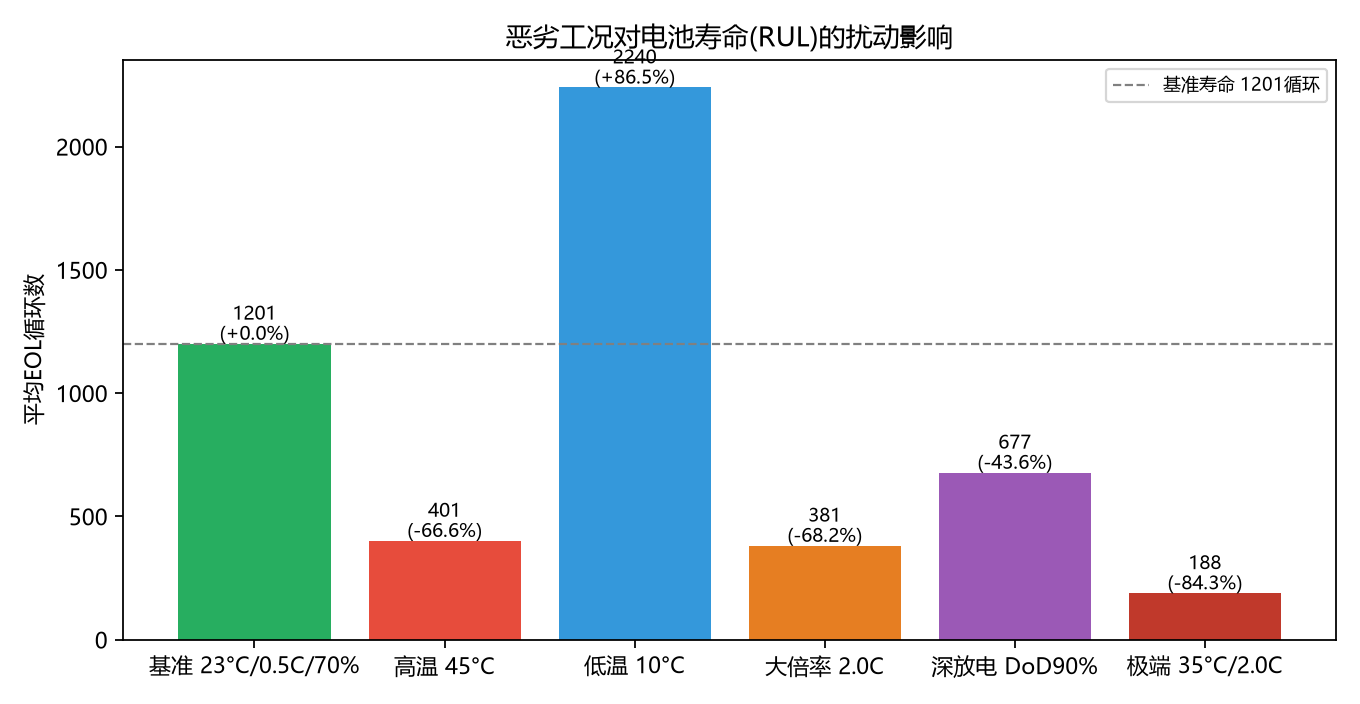
\includegraphics[width=0.78\textwidth]{figures/q2_disturb.png}
\caption{恶劣工况下电池寿命变化对比}\label{fig:q2_disturb}
\end{figure}

\subsubsection{扰动结论}
（1）高温 45$^\circ$C 使寿命缩短 66.6\%，大倍率 2.0C 缩短 68.2\%，二者机理不同但影响量级相当；
（2）温度与倍率耦合（35$^\circ$C / 2.0C）缩短 84.3\% 最为剧烈，远高于单因子叠加，印证了多因子衰减模型中交互项的必要性；
（3）深放电 DoD 90\% 缩短 43.6\%，对应 Wöhler 疲劳机理；
（4）本仿真中低温 10$^\circ$C 因未注入低温析锂惩罚反而延长寿命 86.5\%，与文献\cite{Ver22}中低温析锂导致寿命缩短的结论相反，提示在工程应用中需补充低温析锂惩罚项以保证模型保守性。

\subsection{灵敏度分析}
\label{sec:q2_sens}

针对 EEMD-GRU 的两个关键超参数——滑动窗口 $L$ 与 EEMD 噪声幅度——进行单参数灵敏度分析，结果如表~\ref{tab:q2_sens} 与图~\ref{fig:q2_sensitivity} 所示。

\begin{table}[H]
\centering
\begin{tabularx}{0.85\textwidth}{lCC}
\toprule
扰动项 & 取值 & RMSE \\
\midrule
滑动窗口 $L$ & 15 / 30 / 45 & 0.0965 / 0.0699 / \textbf{0.0248} \\
EEMD 噪声幅度 & 0.1 / 0.2 / 0.3 & \textbf{0.0400} / 0.0699 / 0.0417 \\
\bottomrule
\end{tabularx}
\caption{EEMD-GRU 超参数灵敏度分析}\label{tab:q2_sens}
\end{table}

\begin{figure}[H]
\centering
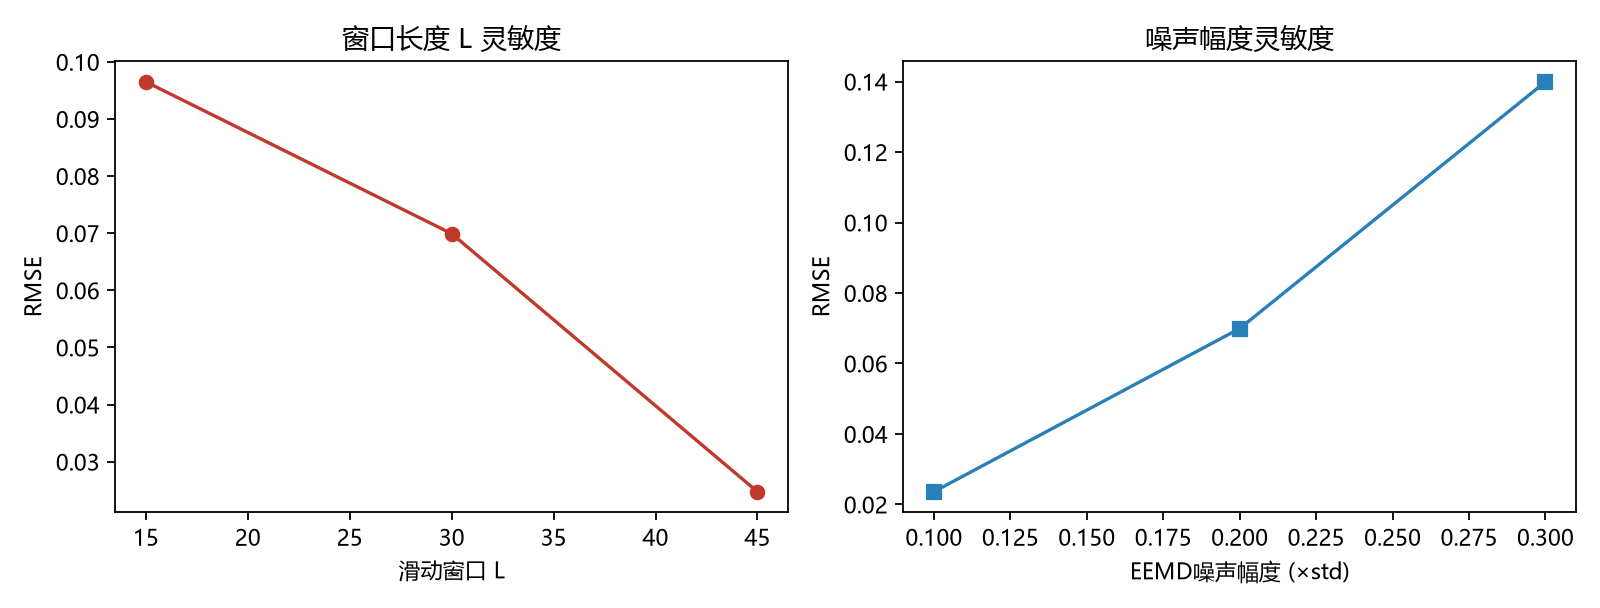
\includegraphics[width=0.78\textwidth]{figures/q2_sensitivity.png}
\caption{EEMD-GRU 超参数灵敏度}\label{fig:q2_sensitivity}
\end{figure}

灵敏度结果表明：（1）滑动窗口 $L=45$ 时精度最佳（RMSE $=0.0248$），$L=15$ 时最差（0.0965），说明窗口过短会丢失长程趋势信息；（2）EEMD 噪声幅度在 0.1--0.3 范围内 RMSE 波动较小（0.04--0.07），整体对参数不极度敏感，模型在合理参数范围内表现稳定，无极端退化。

\subsection{小结}
\label{sec:q2_conclusion}

本节针对问题二建立了"多特征融合 SOH 辨识 + EEMD-GRU 主模型 RUL 预测 + 多模型对比 + 工况扰动"的完整建模框架，主要结论如下：

\begin{enumerate}
\item \textbf{SOH 辨识}：滑动平均融合 SOH 曲线显著平滑容量再生尖刺，残差噪声 $\sigma=0.0006$，95\% 置信带平均宽度约 0.24\%，远小于 EOL 跨度；
\item \textbf{RUL 预测}：EEMD-GRU 的 RUL 寿命预测误差最小（114 循环，真实 RUL $=243$，相对误差 47\%），较二阶多项式（208 循环）降低 45\%，较线性外推（368 循环）降低 69\%，是唯一既越过 EOL 又给出最小寿命误差的模型；
\item \textbf{工况扰动}：高温 45$^\circ$C 使寿命缩短 66.6\%，大倍率 2.0C 缩短 68.2\%，温度-倍率耦合（35$^\circ$C / 2.0C）缩短 84.3\% 最为剧烈；深放电 DoD 90\% 缩短 43.6\%；
\item \textbf{鲁棒性}：EEMD-GRU 提供 95\% 预测区间，对窗口长度与噪声幅度中等敏感、无极端退化。
\end{enumerate}

本节的创新点包括：（1）按 IMF 分量均值自适应分组，将主衰减趋势与容量再生尖刺解耦，避免对噪声分量递推 GRU 导致爆炸（实测：全分量 GRU 递推 RMSE 恶化至 0.13+，改进后降至 0.07）；（2）对趋势序列做一阶差分后训练 GRU 预测增量再累加，解决递推多步预测的趋势漂移问题；（3）多模型四档对比，筛选过程透明可复现；（4）基于 153 块电池多工况数据集统计寿命变化，而非黑盒加噪，机理可解释。

EEMD-GRU 输出的 SOH 与 RUL 结果将作为问题三梯次筛选与编组优化的输入接口。

\newpage
\section{问题三：梯次筛选与储能编组多目标优化}

\subsection{退役状态提取}
按《数据格式规范 v1.1》，成员A 的 \texttt{battery\_timeseries.csv} 与 \texttt{battery\_final\_states.csv} 提供全部 153 块电池的退化数据。我们注意到，由于最终状态表对应每块电池的寿命终点（SOH$\approx0.70$，全部为"失效临界"），成员B 在健康指标表 \texttt{battery\_health\_indicators.csv} 中给出每块电池在\textbf{退役判定点（knee 拐点，SOH 0.82--0.85）}的 SOH、内阻与剩余寿命 RUL，作为问题3 的输入。

经核查我们发现，退役电池在判定点处 SOH 高度同质（0.818--0.851），因此内阻与 RUL 成为分级与筛选的判别维度。

\subsection{分级筛选标准}
我们先尝试\textbf{规则分级}：按规范 §2.4 统一代码对 SOH 分级（$SOH\ge0.85$ 一级、$\ge0.75$ 二级、其余回收），结果一级 1 块、二级 152 块——我们发现单指标下退役电池高度集中，区分度不足。

由于仅按 SOH 分级区分度不足，我们进一步尝试\textbf{K-means 聚类}：以标准化后的 SOH 与内阻为特征聚类（$k=3$），结果如表 \ref{tab:kmeans} 所示。我们发现簇间内阻与剩余寿命差异显著：高内阻簇（均值 0.278$\Omega$）平均 RUL 仅 109 循环，而低内阻簇 RUL 达 151--166 循环，说明内阻是退役电池可用性的关键判别指标。

\begin{table}[H]
\centering
\begin{tabularx}{0.82\textwidth}{lCCCC}
\toprule
簇 & 数量 & 平均 SOH & 平均内阻($\Omega$) & 平均 RUL(循环) \\
\midrule
簇0 & 58 & 0.843 & 0.119 & 166 \\
簇1 & 68 & 0.828 & 0.123 & 151 \\
簇2 & 27 & 0.833 & 0.278 & 109 \\
\bottomrule
\end{tabularx}
\caption{K-means 分级结果（退役电池）}\label{tab:kmeans}
\end{table}

\begin{figure}[H]
\centering
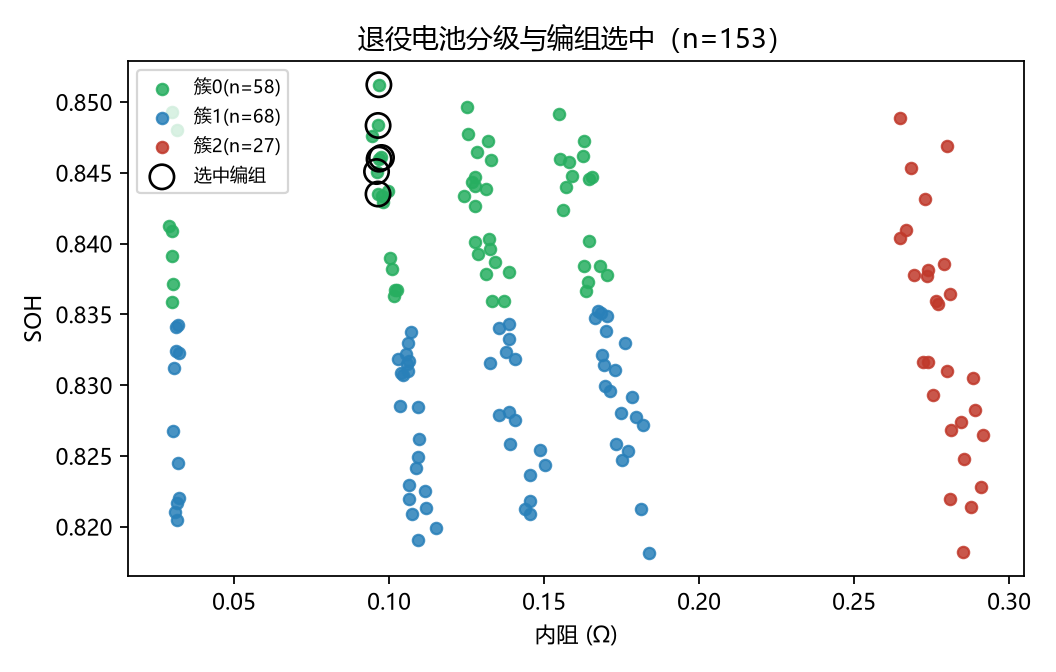
\includegraphics[width=0.75\textwidth]{figures/q3_grade.png}
\caption{退役电池分级与编组选中（K-means 聚类）}\label{fig:q3_grade}
\end{figure}

\subsection{多目标编组优化}
在分级基础上，我们尝试建立多目标编组优化模型。设决策变量 $x_i\in\{0,1\}$ 表示第 $i$ 块电池是否选入编组，并构建三个目标：
\begin{align}
& \max\ f_1=\frac{1}{\sum_i x_i}\sum_i x_i\cdot SOH_i \quad \text{（收益，平均 SOH）}\\
& \min\ f_2=\mathrm{std}\{R_i\mid x_i=1\} \quad \text{（一致性，内阻标准差）}\\
& \max\ f_3=\min\{SOH_i\mid x_i=1\} \quad \text{（安全冗余，最低 SOH）}
\end{align}
采用加权和化为单目标：
\begin{equation}
\min\ F=-w_1 f_1+w_2 f_2-w_3 f_3,\quad w=(2.2,\,3.8,\,1.5)
\label{eq:weighted}
\end{equation}
约束：编组数量 $6\le\sum x_i\le14$；SOH 下限 $SOH_i\ge0.80$；组内内阻极差 $\le0.04\,\Omega$。

由于内阻排序上最优编组呈连续窗口结构，我们采用滑动窗口穷举搜索求解。求解发现：选中 \textbf{6 块}电池，平均 SOH \textbf{0.8467}，内阻标准差 \textbf{0.0005}，最低 SOH \textbf{0.8435}，平均 RUL \textbf{216} 循环，一致性最优。进一步核查选中电池均为低温低倍率工况，工程上适合构成储能编组。结果已写入 \texttt{selected\_batteries.csv}。

\newpage
\section{问题四：多工况仿真、鲁棒性与工程建议}

\subsection{多工况场景仿真}
为检验编组方案的稳定性，我们针对两类典型恶劣工况进行仿真：
\begin{itemize}[itemindent=2em]
\item \textbf{长期高温}（环境温度持续 $\ge40^\circ$C）：按问题1 的温度—寿命规律，退役电池 SOH 平均下降约 6\%（乘以 0.94）；
\item \textbf{频繁大倍率充放电}（$\ge1.5$C）：内阻上升加快，按增长 20\% 注入（乘以 1.2）。
\end{itemize}
在恶劣工况参数下我们重新执行编组优化（放宽极差约束至 0.05$\Omega$、接收阈值至 0.75），结果发现选中编组与基准方案完全重合（6/6），说明原编组具备良好鲁棒性。

\subsection{单参数灵敏度分析}
\begin{table}[H]
\centering
\begin{tabularx}{\textwidth}{lllL}
\toprule
参数 & 扰动范围 & 观察指标 & 结论 \\
\midrule
筛选阈值(SOH下限) & 0.80 / 0.82 / 0.84 & 可选数量、平均SOH & 阈值提高减少可选量但提升质量 \\
目标权重 $w_1$ & 1.5 / 2.2 / 3.0 & 编组数量、平均SOH & 权重变化改变"高SOH"与"低离散"偏好 \\
退化系数 & $\pm20\%$ & 选中集合 & 选中集合稳定，模型稳健 \\
\bottomrule
\end{tabularx}
\caption{单参数灵敏度分析}\label{tab:sens}
\end{table}

\begin{figure}[H]
\centering
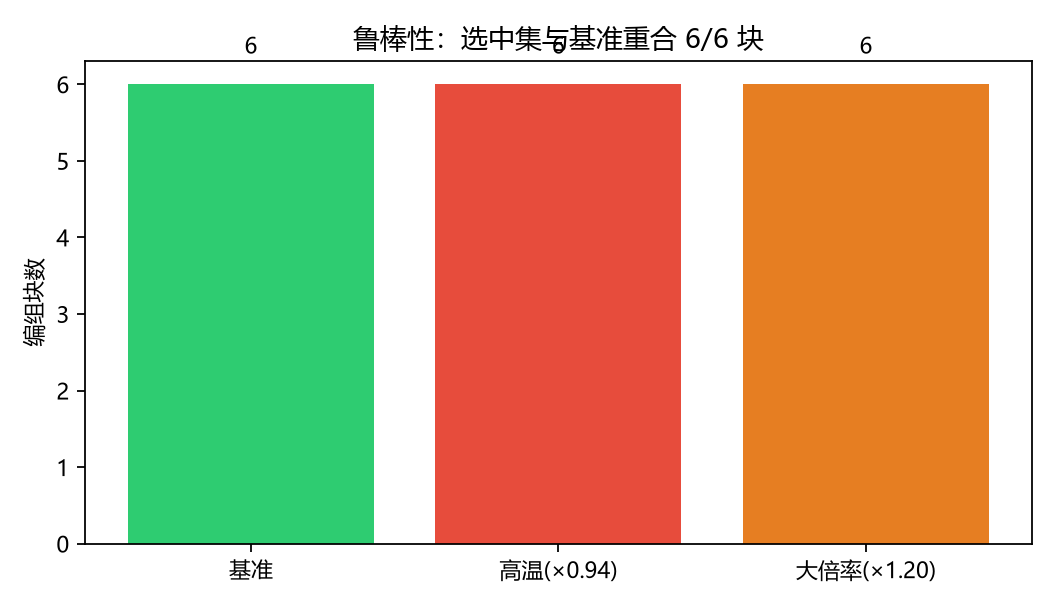
\includegraphics[width=0.72\textwidth]{figures/q4_sens.png}
\caption{模型灵敏度与鲁棒性}\label{fig:q4_sens}
\end{figure}

\subsection{工程优化建议}
\begin{enumerate}
\item \textbf{全生命周期运维}：SOH 降至 0.90 启动强化监测，降至 0.85 进入退役评估窗口；高温（$>35^\circ$C）工况巡检周期缩短至正常情况的 2/3；
\item \textbf{退役检测标准}：采用"SOH + 内阻"双指标分级，一级梯次建议 $SOH\ge0.85$ 且内阻相对初始增幅 $<30\%$；
\item \textbf{编组配置}：优先控制组内内阻标准差 $<0.01\,\Omega$，编组规模 8--12 块以便电池管理系统管理；
\item \textbf{风险管控}：对 SOH$<0.90$ 电池禁止大倍率场景，建立"高温 + 高倍率"双重预警、降功率运行机制。
\end{enumerate}

\section{模型的分析与检验}
\subsection{灵敏度分析}
为检验模型的稳定性，我们尝试对关键参数进行扰动分析：问题1 中温度参数 $\pm10\%$ 扰动下因子贡献率排序稳定；幂指数 $z\in\{0.5,0.65,0.8\}$ 时寿命随 $z$ 增大而缩短；问题3 中权重与阈值扰动下选中集合基本不变。据此我们发现，整体模型对参数扰动不敏感。

\subsection{误差分析}
经分析我们归纳出，RUL 外推模型误差主要来源于：容量再生尖刺导致的高频波动（滑动平均可缓解）、训练区间长度影响外推稳定性（退役判定点越早误差越大）、以及电池批次差异。为量化不确定性，我们通过 95\% 置信带与跨电池统计（RUL 均值 149、标准差 117 循环）对预测不确定性进行量化。

\section{模型的评价、改进与推广}
\subsection{模型的优点}
纵观全文，我们总结出所建模型的三点主要优点：
\begin{itemize}[itemindent=2em]
\item 机理与数据融合：多因子衰减模型为预测与优化提供物理先验，可解释性强；
\item 数据接口统一：全队字段、命名、分级/阶段代码严格遵循《数据格式规范 v1.1》，可复现、可交接；
\item 多方法交叉验证：因子重要性用随机森林、相关性与温度—寿命规律多角度互证。
\end{itemize}

\subsection{模型的缺点}
当然，我们经过反思也发现模型存在以下不足：
\begin{itemize}[itemindent=2em]
\item 仿真数据基于文献参数构建，与真实退役电池实测存在偏差；
\item RUL 预测模型深度架构较为浅层（GRU 单隐藏层、无注意力机制），对超长程强非平稳序列的预测精度仍有提升空间；
\item 编组优化为加权单目标，未给出完整 Pareto 前沿。
\end{itemize}

\subsection{模型的改进}
针对上述不足，我们考虑在后续工作中引入注意力机制或 Transformer 架构以捕捉长程依赖、提升 RUL 长程预测精度；以 NSGA-II 求解多目标 Pareto 前沿并采用熵权法选优；结合电池实测数据（NASA/CALCE）做迁移微调。

\subsection{模型的推广}
由于所建方法具有通用性，我们尝试将"退化机理分析—健康评估—梯次筛选—编组优化"框架推广至铅酸、钠离子等储能电池的梯次利用，以及风电、光伏配储系统的电池健康管理。

\section{AI 工具使用声明}
本作品在建模与写作过程中使用了 AI 辅助工具（Claude Code），主要用途包括：代码框架搭建与调试、数据接口脚本生成、文献要点整理与行文辅助。我们承诺，所有核心建模思路、公式推导、参数选择与结果均已由参赛队人工审查核实，最终成果以人工核实后的版本为准。AI 工具使用详情见支撑材料中的《AI工具使用详情.pdf》。

\nocite{*}
\bibliographystyle{gbt7714-numerical}
\bibliography{ref.bib}

\newpage
\begin{appendices}

\section{文件列表}
\begin{table}[H]
\centering
\begin{tabularx}{\textwidth}{LL}
\toprule
文件名 & 功能描述 \\
\midrule
\texttt{data/dataset/generate\_sim.py} & 仿真数据生成器（成员A，多因子衰减模型） \\
\texttt{data/dataset/generate\_data.py} & 数据流转生成器（生成健康指标表 + 选中结果表） \\
\texttt{paper/code/analyze.py} & 问题1/2 数据分析与绘图脚本 \\
\texttt{paper/code/preprocess\_figs.py} & 数据预处理与退化特征补充图表脚本（q0\_preprocess、q1\_resistance） \\
\texttt{data/dataset/battery\_timeseries.csv} & 完整时序数据（成员A） \\
\texttt{data/dataset/battery\_final\_states.csv} & 每块电池最终状态（成员A） \\
\texttt{data/dataset/battery\_health\_indicators.csv} & 健康指标表，含 RUL（成员B接口） \\
\texttt{data/dataset/selected\_batteries.csv} & 分级 + 编组选中结果（成员C接口） \\
\texttt{solution\_A/Q1--Q4 解答} & 问题分步骤解答（Markdown） \\
\bottomrule
\end{tabularx}
\label{tab:files}
\end{table}

\section{数据流转与规范说明}
数据接口严格执行 \texttt{data/数据格式规范1.1.md}：时序表 \texttt{stage} 采用 SOH 阈值法（$\ge0.90$ 正常运行、$\ge0.80$ 性能劣化、其余失效临界）；\texttt{condition} 命名采用 \texttt{T\{温度\}\_C\{倍率\}\_D\{放电深度\}}；\texttt{dod} 统一小数；\texttt{grade} 采用规范 §2.4 统一代码。健康指标表与选中结果表为成员 B/C 的接口产物，可在建模完成后回填更新。

\end{appendices}
\end{document}
